
\documentclass[a4paper,8pt]{extarticle} % extarticle allows to use font size of 8pt.

\usepackage[a4paper, top=1.6cm, bottom=2cm, left=1.6cm, right=1.6cm]{geometry} % Marge reduction.

%% Language specific package
\usepackage[french]{babel}
\frenchbsetup{StandardLists=true} % Necessary to use enumitem with babel/french.

%% Font and typing packages
\usepackage{fontspec}
\setmainfont[
	Ligatures=TeX,
	ItalicFont={Dancing Script},
	BoldItalicFont={Dancing Script}
	]{PT Serif} % default is Latin Modern
\newfontfamily\antiquefont[Ligatures=TeX]{Caslon Antique} % fancy font
\usepackage{microtype}			% Greatly improves general appearance of the text.
\usepackage{SIunits}			% Unit appearance.
\usepackage{xspace}				% Define commands that appear not to eat spaces.
\usepackage{ulem}				% To cross words out. Use \sout{}.

%% Array utilities
\usepackage{array}				% Additionnal options for arrays.
\usepackage{colortbl}			% Additionnal options for coloring arrays.
\usepackage[table]{xcolor}		% Auto alternate grey-white rows.
\usepackage[export]{adjustbox}		% Centered pics in tables

%% List utilities
\usepackage[inline]{enumitem}   % Display inline lists.
\usepackage{etoolbox}           % General utility. Good for lists for instance.
\usepackage{xparse}             % List utilities.
\usepackage{datatool}	% Handling alphabetical order.

%% Frames
\usepackage{framed}				% Boxes.
\usepackage[framemethod=TikZ]{mdframed}% For fancy frames.
\usepackage{tikz}				% For fancy frames.
\usepackage{wrapfig}			% Fancy insertion of pics in text.

%% Page utilities
\usepackage{multicol}			% Allows to divide a part of the page in multiple columns.
	
%% Others
\usepackage{keyval}             % Used to create maps of commands/labels/objects.
	\makeatletter                  % Mandatory for the usage of keyval.
\usepackage{xstring}            % String parsing, cutting, etc.
\usepackage{hyperref} % Links in PDF.


%%% Update of the dotfill command to always get dots

\newcommand{\predotfill}{\penalty0\hbox{}\nobreak}%


%%% Command to avoid typing \xspace when creating a new name macro

\newcommand{\newnamemacro}[2]{\newcommand{#1}{#2}} % \xspace removed for compatibility with alphabetical ordering

%%% Language specific stuff


\newcommand{\translationteam}{\item \og AEnoriel \fg \item \og Anglachel \fg \item \og Astadriel \fg \item \og Batcat \fg \item \og Bigfish \fg \item \og Eru \fg  \item \og Gandarin \fg \item \og Groumbahk \fg \item \og Iluvatar \fg \item \og Mammstein \fg \item \og Shlagrabak \fg \item et beaucoup d'autres...}

\hypersetup{
	pdfauthor={Équipe de traduction française de T9A},
	pdfsubject={Règles pour le jeu Batailles Fantastiques : Le 9\ieme{} Âge},
}

%%% Commands %%%

\ifdef{\isitanAB}{

\newcommand{\addtosortedlist}[1]{%
	\protected@edef\textarg{#1}%
	\protected@edef\textwithoutspaces{\expandafter\removespaces\expandafter{\textarg}}%
	\substitute\textwithoutspaces{É}{E}% Most used special characters of the language, and equivalent for alphabetical ordering
	\substitute\textwithoutspaces{È}{E}%
	\substitute\textwithoutspaces{Ê}{E}%
	\substitute\textwithoutspaces{é}{e}%
	\substitute\textwithoutspaces{è}{e}%
	\substitute\textwithoutspaces{ê}{e}%
	\substitute\textwithoutspaces{À}{A}%
	\substitute\textwithoutspaces{à}{a}%
	\substitute\textwithoutspaces{ù}{u}%
	\expandafter\sortitem\expandafter[\textwithoutspaces]{#1}%
}%

\newcommand{\pts}[1]{% First step is to remove spaces if there are some
	\def\numberwithoutspaces{\expandafter\removespaces\expandafter{#1}}%
	% Next step is getting rid of formatting if there are any (bold, color, ...)
	\pdfstringdef\cleannumber{\numberwithoutspaces}%
	% Now we can try if it is 1 or not
	\expandafter\ifstrequal\expandafter{\cleannumber}{1}{#1~\labels@point}{%
	\expandafter\ifstrequal\expandafter{\cleannumber}{0.5}{0,5~\labels@point}{%
	\expandafter\ifstrequal\expandafter{\cleannumber}{1.5}{1,5~\labels@point}{%
	#1~\labels@points}}}%
}

}{}

% Dark gods
\newcommand{\dchange}{Changement}
\newcommand{\dlust}{Luxure}
\newcommand{\pestilence}{Pestilence}
\newcommand{\wrath}{Courroux}
\newcommand{\truechaos}{Chaos Primordial}


% Nothing to edit here

\ifdef{\isitanAB}{

\newcommand{\alliancepts}[1]{
\ifsubstring{#1}{\free}{%
		\free{}%
	}{%
	\ifsubstring{#1}{\permodel}{%
		\splitatinf{#1}\myoption\myvalue%
		\pts{\myvalue}\permodel{}%
	}{%
	\pts{#1}
	}}
}

% You might wanna change the order of the gods - advanced user
\newcommand{\allianceoptions}[1]{%
	\defallianceoptions{#1}%
	\unitentryformat{\labels@allianceoptions\spacebeforecolon{}:}\newline
	\expandafter\ifblank\expandafter{\allianceoptions@introsentence}{}{\noindent\allianceoptions@introsentence{}\spacebeforecolon{}:}
	
	\expandafter\ifblank\expandafter{\allianceoptions@wrath}{
		\setlength{\columnseprule}{0.5pt}
		\renewcommand{\columnseprulecolor}{\color{black!30}}
		\vspace*{-0.2cm}\begin{multicols}{3}\raggedcolumns
		
			\begin{center}
			\noindent\dchange{}
			
			\noindent\alliancepts{\allianceoptions@change}
			\vspace*{-0.3cm}
			\end{center}
		
		\columnbreak
		
			\begin{center}
			\noindent\dlust{}
			
			\noindent\alliancepts{\allianceoptions@lust}
			\vspace*{-0.3cm}
			\end{center}
		
		\columnbreak

			\begin{center}
			\noindent\pestilence{}
			
			\noindent\alliancepts{\allianceoptions@pestilence}
			\vspace*{-0.3cm}
			\end{center}
			
		\end{multicols}
		\setlength{\columnseprule}{0pt}	
	}{
		\setlength{\columnseprule}{0.5pt}
		\renewcommand{\columnseprulecolor}{\color{black!30}}
		\vspace*{-0.2cm}\begin{multicols}{4}\raggedcolumns
		
			\begin{center}
			\noindent\dchange{}
			
			\noindent\alliancepts{\allianceoptions@change}
			\vspace*{-0.3cm}
			\end{center}
		
		\columnbreak

			\begin{center}
			\noindent\wrath{}
			
			\noindent\alliancepts{\allianceoptions@wrath}
			\vspace*{-0.3cm}
			\end{center}
		
		\columnbreak
		
			\begin{center}
			\noindent\dlust{}
			
			\noindent\alliancepts{\allianceoptions@lust}
			\vspace*{-0.3cm}
			\end{center}
		
		\columnbreak

			\begin{center}
			\noindent\pestilence{}
			
			\noindent\alliancepts{\allianceoptions@pestilence}
			\vspace*{-0.3cm}
			\end{center}
			
		\end{multicols}
		\setlength{\columnseprule}{0pt}
	}
}

}{}


%%% Labels %%%

% Profile

\newcommand{\labels@M}{M}
\newcommand{\labels@WS}{CC}
\newcommand{\labels@BS}{CT}
\newcommand{\labels@S}{F}
\newcommand{\labels@T}{E}
\newcommand{\labels@W}{PV}
\newcommand{\labels@I}{I}
\newcommand{\labels@A}{A}
\newcommand{\labels@Ld}{Cd}
\newcommand{\labels@Invocation}{Invocation} % For Vampire Covenant profiles
\newcommand{\labels@roundbase}{rond} % printed after XX mm for round bases

\newcommand{\Strength}{Force}

% Technical

\newcommand{\labels@range}{Portée}
\newcommand{\labels@point}{pt}
\newcommand{\labels@points}{pts}
\newcommand{\labels@only}{uniquement}
\newcommand{\labels@magic}{Magie}
\newcommand{\labels@pathsused}{Génère ses sorts dans la Discipline}
\newcommand{\labels@model}{figurine}
\newcommand{\labels@models}{figurines}
\newcommand{\labels@Singlemodel}{Figurine \textbf{seule}}

% Unit entry labels

\newcommand{\labels@basesize}{Socle}
\newcommand{\labels@trooptype}{Type de troupe}
\newcommand{\labels@specialrules}{Règles Spéciales}
\newcommand{\labels@alignment}{Allégeance}
\newcommand{\labels@alliance}{Allégeance}
\newcommand{\labels@allianceoptions}{Options d'Allégeance}
\newcommand{\labels@greenhiderace}{Race de Peaux Vertes}
\newcommand{\labels@equipment}{Équipement}
\newcommand{\labels@weapons}{Armes}
\newcommand{\labels@armour}{Armure}
\newcommand{\labels@options}{Options}
\newcommand{\labels@commandgroup}{État-Major}
\newcommand{\labels@charactermounts}{Montures de Personnages}
\newcommand{\labels@mounts}{Montures}
\newcommand{\labels@mount}{Monture}
\newcommand{\labels@specialequipment}{Équipement Spécial}

% Command groups

\newcommand{\labels@champion}{Champion}
\newcommand{\labels@standardbearer}{Porte-Étendard}
\newcommand{\labels@musician}{Musicien}
\newcommand{\labels@singlebannerallowance}{Une seule unité de ce type peut prendre une Bannière Magique}
\newcommand{\labels@condsinglebannerallowance}{Une seule unité de ce type peut prendre une Bannière Magique si}
\newcommand{\labels@bannerallowance}{Bannière Magique}
\newcommand{\labels@veteranstandardbearer}{Peut devenir Porte-Étendard Vétéran}
\newcommand{\labels@championallowance}{Arme Magique}

% Titles

\newcommand{\labels@armylist}{Liste des Troupes}
\newcommand{\labels@lords}{Seigneurs}
\newcommand{\labels@heroes}{Héros}
\newcommand{\labels@coreunits}{Unités de Base}
\newcommand{\labels@specialunits}{Unités Spéciales}
\newcommand{\labels@rareunits}{Unités Rares}
\newcommand{\labels@armywiderules}{Règles Communes de l'Armée}
\newcommand{\labels@armyspecialrules}{Règles Spéciales de l'Armée}
\newcommand{\labels@armoury}{Armurerie}
\newcommand{\labels@magicalitems}{Objets Magiques}
\newcommand{\labels@magicalweapons}{Armes Magiques}
\newcommand{\labels@magicalarmour}{Armures Magiques}
\newcommand{\labels@talismans}{Talismans}
\newcommand{\labels@enchanteditems}{Objets Enchantés}
\newcommand{\labels@arcaneitems}{Objets Cabalistiques}
\newcommand{\labels@magicalbanners}{Bannières Magiques}
\newcommand{\labels@quickrefsheet}{Fiche de Référence}
\newcommand{\labels@changelog}{Change Log}

\newcommand{\labels@lordsInitial}{S}
\newcommand{\labels@heroesInitial}{H}
\newcommand{\labels@coreunitsInitial}{B}
\newcommand{\labels@specialunitsInitial}{S}
\newcommand{\labels@rareunitsInitial}{R}
\newcommand{\labels@mountsInitial}{M}


% Titlepage

\newcommand{\labels@fantasybattles}{Batailles Fantastiques}
\newcommand{\labels@NinthAge}{Le 9\ieme{} Âge}
\newcommand{\labels@armyrules}{Règles de l'Armée}
\newcommand{\labels@frontpagecredits}{%
\labels@fantasybattles{} : \labels@NinthAge{} est un jeu créé et entretenu par la communauté qui met en scène des affrontements de figurines.\newline
Toutes les règles sont disponibles gratuitement sur le site suivant. Vos retours et suggestions sont les bienvenus : \url{http://www.the-ninth-age.com/}
}
\newcommand{\labels@license}{Copyright Creative Commons license : \url{the-ninth-age.com/license.html}}
\newcommand{\labels@tableofcontents}{Sommaire}
\newcommand{\labels@introduction}{%
\begin{center}\noindent{\Largerfontsize\textbf{Note des traducteurs}}\end{center}
\vspace{0.5cm}

Nous souhaitons remercier chaleureusement l'équipe à l'initiative du 9\ieme{} Âge pour leur motivation et leur travail continu pour faire vivre notre passion. Nous espérons que ce jeu saura développer les qualités pour plaire au plus grand nombre et réunir les joueurs, amateurs comme habitués des tournois, autour de règles amusantes et équilibrées, pour finalement s'imposer comme un standard du jeu de figurines. Une grande ambition qui ne pourra s'accomplir que \textbf{grâce à vous}, la communauté, via des retours constructifs, afin de modeler le jeu selon nos désirs. N'étant \textbf{en aucun cas à but lucratif}, le 9\ieme{} Âge part avec un avantage considérable. Les règles des éventuelles nouvelles sorties ne sont pas dictées par le besoin de vendre ces nouveautés. Vous pouvez choisir et acheter vos figurines où bon vous semble, il n'y a pas un unique revendeur toléré. Enfin, vous pouvez être assurés que tant que le 9\ieme{} Âge sera joué, vous disposerez d'un \textbf{support continu et régulier}, celui-ci étant offert par la communauté.

Concernant la traduction en elle-même, nous avons fait de notre mieux pour vous offrir une version de qualité, dont nous espérons qu'elle surpasse celle de la version originale ! Si vous constatez des coquilles, des erreurs, merci de nous les signaler en nous contactant sur le forum du 9\ieme{} Âge, dans le \textbf{sous-forum français} (\url{http://www.the-ninth-age.com/index.php?board/117-french/}). Vous y trouverez aussi les dernières mises à jour. \textbf{En cas de conflit d'interprétation avec la version originale, la version originale fait référence}.

\vspace{0.5cm}
Que ce jeu vous apporte d'innombrables heures de plaisir partagé !

\vspace{1cm}

\ifdef{\translationteam}{
	\begin{multicols}{3}
	\begin{itemize}
		\translationteam
	\end{itemize}
	\end{multicols}
}{}
}
\newcommand{\labels@rulechanges}{% blank ATM
}
\newcommand{\labels@latexcredit}{Document réalisé à l'aide de \LaTeX .}


%%% Technical commands

\newcommand{\only}[1]{(#1 uniquement)}
\newcommand{\free}{gratuit}
\newcommand{\upto}{jusqu'à}
\newcommand{\Upto}{Jusqu'à}
\newcommand{\unlimited}{pas de limite}
\newcommand{\permodel}{/fig.}
\newcommand{\listlastchoice}{ ou}
\newcommand{\notif}[1]{(pas #1)}
\newcommand{\wordand}{et}
\newcommand{\wordwith}{avec}
\newcommand{\ifNmodelsorless}[1]{(#1 figurines ou moins)}
\newcommand{\unitwith}{unité avec}
\newcommand{\From}{De} % From ... to ... models
\newcommand{\wordto}{à}
\newcommand{\wordAll}{Tous}
\newcommand{\spacebeforecolon}{ } % French put a space before colons
\newcommand{\minprice}{Coût min. :}
\newcommand{\mincostfor}{Coût min. pour}
\newcommand{\maxunitsize}{Taille max.}
\newcommand{\additionalfigscost}{Les figurines additionnelles coûtent}


%%% Special rules %%%

\newcommand{\ambush}{Embuscade}
\newcommand{\armourpiercing}[1]{Perforant\ifblank{#1}{}{ (#1)}}
\newcommand{\bodyguard}[1]{Garde du Corps\ifblank{#1}{}{ (#1)}}
\newcommand{\breathweapon}[1]{Attaque de Souffle\ifblank{#1}{}{ (#1)}}
\newcommand{\channel}{Canalisation}
\newcommand{\crushattack}{Attaque Écrasante}
\newcommand{\daemonicinstability}{Instabilité Démoniaque}
\newcommand{\devastatingcharge}{Charge Dévastatrice}
\newcommand{\distracting}{Distrayant}
\newcommand{\divineattacks}{Attaques Divines}
\newcommand{\engineer}{Ingénieur}
\newcommand{\ethereal}{Éthéré}
\newcommand{\fastcavalry}{Cavalerie Légère}
\newcommand{\fear}{Peur}
\newcommand{\fightinextrarank}{Combat avec un Rang Supplémentaire}
\newcommand{\fireborn}{Né du Feu}
\newcommand{\flamingattacks}{Attaques Enflammées}
\newcommand{\flammable}{Inflammable}
\newcommand{\frenzy}{Frénésie}
\newcommand{\fly}[1]{Vol\ifblank{#1}{}{ (#1)}}
\newcommand{\grindingattacks}[1]{Attaques de Broyage\ifblank{#1}{}{ (#1)}}
\newcommand{\hardtarget}{Camouflé}
\newcommand{\hatred}{Haine}
\newcommand{\hellfire}{Feu Démoniaque}
\newcommand{\hidden}{Caché}
\newcommand{\holyattacks}{Attaques Divines} % deprecated, still has to be filled. same as Divine Attacks.
\newcommand{\immunetopsychology}{Immunisé à la Psychologie}
\newcommand{\impacthits}[1]{Touches d'Impact\ifblank{#1}{}{ (#1)}}
\newcommand{\insignificant}{Insignifiant}
\newcommand{\largetarget}{Grande Cible}
\newcommand{\lethalstrike}{Coup Fatal}
\newcommand{\lightningattacks}{Attaques Foudroyantes}
\newcommand{\lightningreflexes}{Réflexes Foudroyants}
\newcommand{\lighttroops}{Troupe Légère}
\newcommand{\magicresistance}[1]{Résistance à la Magie\ifblank{#1}{}{ (#1)}}
\newcommand{\magicalattacks}{Attaques Magiques}
\newcommand{\metalshifting}{Fusion du Métal}
\newcommand{\moveorfire}{Mouvement ou Tir}
\newcommand{\multipleshots}[1]{Tirs Multiples\ifblank{#1}{}{ (#1)}}
\newcommand{\multiplewounds}[2]{Blessures Multiples\ifblank{#1}{}{ (#1\ifblank{#2}{)}{, #2)}}}
\newcommand{\notaleader}{Pas un Meneur}
\newcommand{\otherworldly}{D'Outre-Monde}
\newcommand{\pathmaster}[1]{Maître de la Voie\ifblank{#1}{}{ (#1)}}
\newcommand{\poisonedattacks}{Attaques Empoisonnées}
\newcommand{\quicktofire}{Tir Rapide}
\newcommand{\randommovement}[1]{Mouvement Aléatoire\ifblank{#1}{}{ (#1)}}
\newcommand{\randomattacks}[1]{Attaques Aléatoires\ifblank{#1}{}{ (#1)}}
\newcommand{\regeneration}[1]{Régénération\ifblank{#1}{}{ (#1+)}}
\newcommand{\reload}{Rechargez !}
\newcommand{\requirestwohands}{Arme à deux Mains}
\newcommand{\scythes}{Faux}
\newcommand{\scout}{Éclaireur}
\newcommand{\scouts}{Éclaireurs}
\newcommand{\stomp}[1]{Piétinement\ifblank{#1}{}{ (#1)}}
\newcommand{\strider}[1]{Guide\ifblank{#1}{}{ (#1)}}
\newcommand{\stubborn}{Tenace}
\newcommand{\stupidity}{Stupidité}
\newcommand{\skirmisher}{Tirailleur}
\newcommand{\skirmishers}{Tirailleurs}
\newcommand{\sweepingattack}{Attaque au Passage}
\newcommand{\swiftstride}{Course Rapide}
\newcommand{\thunderouscharge}{Charge Tonitruante}
\newcommand{\terror}{Terreur}
\newcommand{\toxicattacks}{Attaques Toxiques}
\newcommand{\unbreakable}{Indémoralisable}
\newcommand{\undead}{Mort-Vivant}
\newcommand{\unstable}{Instable}
\newcommand{\unwieldy}{Encombrant}
\newcommand{\vanguard}{Avant-Garde}
\newcommand{\volleyfire}{Tir de Volée}
\newcommand{\warplatform}{Plateforme de Guerre}
\newcommand{\wardsave}[1]{Sauvegarde Invulnérable\ifblank{#1}{}{ (#1+)}}
\newcommand{\weaponmaster}{Maître d'Ar\-mes}
\newcommand{\wizardconclave}[1]{Conclave de Sorciers\ifblank{#1}{}{ (#1)}}


%%% Magic %%%


% General

\newcommand{\Pathof}{Voie}

\newcommand{\battle}{Commune}

\newcommand{\anyofthebattlemagic}{dans n'importe laquelle des Voies Communes}
\newcommand{\ONLYanyofthebattlemagic}{Commune de votre choix}

\newcommand{\magiclevel}[1]{\ifnumcomp{#1}{<}{3}{Apprenti Magicien}{Maître Magicien} Niveau #1}
\newcommand{\Level}{Niveau}

\newcommand{\wizard}{Magicien}
\newcommand{\wizards}{Magiciens}

\newcommand{\learnedspell}{Sort Appris}
\newcommand{\learnedspells}{Sorts Appris}
\newcommand{\attributespell}{Attribut de la Voie}
\newcommand{\attributespells}{Attributs de la Voie}
\newcommand{\attributespellnumber}{A}
\newcommand{\traitspell}{Sort Caractéristique}
\newcommand{\traitspells}{Sorts Caractéristiques}
\newcommand{\traitspellnumber}{C}


\newcommand{\boundspell}[1]{Objet de Sort\ifblank{#1}{}{, Puissance #1}}
\newcommand{\boundspells}[1]{Objets de Sort\ifblank{#1}{}{, Puissance #1}}

% Casting Vocabulary

\newcommand{\lostfocus}{Perte de Concentration}
\newcommand{\miscast}{Fiasco}
\newcommand{\miscasts}{Fiascos}
\newcommand{\overwhelmingpower}{Pouvoir Irrésistible}

\newcommand{\breachintheveil}{Brèche dans le Voile}
\newcommand{\catastrophicdetonation}{Explosion Catastrophique}
\newcommand{\witchfire}{Feu de Sorcières}
\newcommand{\sorcerousbacklash}{Contrecoup Magique}
\newcommand{\amnesia}{Amnésie}

% Spell Types

\newcommand{\augment}{Amélioration}
\newcommand{\hex}{Malédiction}
\newcommand{\universal}{Universel}
\newcommand{\missile}{Projectile}
\newcommand{\damage}{Dégâts}
\newcommand{\direct}{Direct}
\newcommand{\focused}{Focalisé}
\newcommand{\vortex}{Vortex}
\newcommand{\ground}{Marqueur}
\newcommand{\linetemplate}{Gabarit de Ligne}
\newcommand{\specialTYPE}{Spécial}
\newcommand{\aura}{Aura}
\newcommand{\castersunit}{Unité du Lanceur}
\newcommand{\caster}{Lanceur}

\newcommand{\template}{Gabarit}

% Spell Durations

\newcommand{\lastsoneturn}{Dure un Tour}
\newcommand{\instant}{Immédiat}
\newcommand{\permanent}{Permanent}
\newcommand{\remainsinplay}{Reste en Jeu}


% Battle Magic

\newcommand{\alchemy}{de l'Alchimie}
\newcommand{\alchemyattribute}{Édit de Fer}
\newcommand{\alchemysignature}{Métal Fondu}
\newcommand{\alchemyspellone}{Lames Enchantées}
\newcommand{\alchemyspelltwo}{Corrosion Rampante}
\newcommand{\alchemyspellthree}{Manteau de Vif-Argent}
\newcommand{\alchemyspellfour}{Pieu d'Argent}
\newcommand{\alchemyspellfive}{Fléau de l'Acier}
\newcommand{\alchemyspellsix}{Transmutation en Or}

\newcommand{\death}{de la Mort}
\newcommand{\deathattribute}{Nuage de Désespoir}
\newcommand{\deathsignature}{Le Baiser de la Faucheuse}
\newcommand{\deathspellone}{Malédiction du Mortel}
\newcommand{\deathspelltwo}{Esprits Dévorants}
\newcommand{\deathspellthree}{Sangsue Psychique}
\newcommand{\deathspellfour}{Moisson d’Âmes}
\newcommand{\deathspellfive}{L’Abîme aussi te Regarde...}
\newcommand{\deathspellsix}{Maelström d’Âmes}

\newcommand{\fire}{du Feu}
\newcommand{\fireattribute}{Feu Déchaîné}
\newcommand{\firesignature}{Boule de Feu}
\newcommand{\firespellone}{Cascade Ardente}
\newcommand{\firespelltwo}{Épées Flamboyantes}
\newcommand{\firespellthree}{Jet de Flammes}
\newcommand{\firespellfour}{Traits Enflammés}
\newcommand{\firespellfive}{Remparts Incandescents}
\newcommand{\firespellsix}{Souffler sur les Braises}

\newcommand{\heavens}{des Cieux}
\newcommand{\heavensattribute}{Second Sceau}
\newcommand{\heavenssignature}{Aquilon}
\newcommand{\heavensspellone}{Bourrasque}
\newcommand{\heavensspelltwo}{Choc Foudroyant}
\newcommand{\heavensspellthree}{Conjonction Astrale}
\newcommand{\heavensspellfour}{Fléau du Ponant}
\newcommand{\heavensspellfive}{Déluge d'Éclairs}
\newcommand{\heavensspellsix}{Appel de la Comète}

\newcommand{\light}{de la Lumière}
\newcommand{\lightattribute}{Lumière Gardienne}
\newcommand{\lightsignature}{Éclat Brûlant}
\newcommand{\lightspellone}{Bouclier Protecteur}
\newcommand{\lightspelltwo}{Étincelle de Courage}
\newcommand{\lightspellthree}{Vitesse Fulgurante}
\newcommand{\lightspellfour}{Toile Scintillante}
\newcommand{\lightspellfive}{Distorsion Temporelle}
\newcommand{\lightspellsix}{Bannissement Divin}

\newcommand{\nature}{de la Nature}
\newcommand{\natureattribute}{Souffle de Vie}
\newcommand{\naturesignature}{Eaux Vivifiantes}
\newcommand{\naturespellone}{Maître de la Terre}
\newcommand{\naturespelltwo}{Le Trône de Chêne}
\newcommand{\naturespellthree}{Esprits des Bois}
\newcommand{\naturespellfour}{Croissance Estivale}
\newcommand{\naturespellfive}{Peau Rocailleuse}
\newcommand{\naturespellsix}{Créatures Souterraines}

\newcommand{\shadows}{des Ombres}
\newcommand{\shadowsattribute}{Course Parmi les Ombres}
\newcommand{\shadowssignature}{Miasmes Obscurs}
\newcommand{\shadowsspellone}{Orbe de Noirceur}
\newcommand{\shadowsspelltwo}{Partir en Fumée}
\newcommand{\shadowsspellthree}{Expérience de Mort Imminente}
\newcommand{\shadowsspellfour}{Char Vaporeux}
\newcommand{\shadowsspellfive}{Ombres Dévorantes}
\newcommand{\shadowsspellsix}{Scalpel Psychique}

\newcommand{\wilderness}{de la Sauvagerie}
\newcommand{\wildernessattribute}{La Chasse Sauvage}
\newcommand{\wildernesssignature}{La Bête qui Sommeille}
\newcommand{\wildernessspellone}{Essaim d’Insectes}
\newcommand{\wildernessspelltwo}{Rage Intérieure}
\newcommand{\wildernessspellthree}{Pieu de Rougebois}
\newcommand{\wildernessspellfour}{Calamité des Bois Sauvages}
\newcommand{\wildernessspellfive}{Tempête Furieuse}
\newcommand{\wildernessspellsix}{Métamorphose
Monstrueuse}

\newcommand{\eightpaths}{Octuple}



% Army Specific Magic

\newcommand{\butchery}{de la Boucherie}
\newcommand{\butcheryattribute}{Sang de Kholag}
\newcommand{\butcherysignature}{Briseur de Dents}
\newcommand{\butcheryspellone}{Buveur de Moelle}
\newcommand{\butcheryspelltwo}{Festin de Tripaille}
\newcommand{\butcheryspellthree}{Concasseur d’Os}
\newcommand{\butcheryspellfour}{Gobeur de Cervelle}
\newcommand{\butcheryspellfive}{Cœur de Troll}
\newcommand{\butcheryspellsix}{Gosier de Géant}

\newcommand{\change}{du Changement}
\newcommand{\changeattribute}{Vent du Changement}
\newcommand{\changesignature}{Feu Azur}
\newcommand{\changespellone}{Feu Rose}
\newcommand{\changespelltwo}{Vague du Changement}
\newcommand{\changespellthree}{Secrets Volés}
\newcommand{\changespellfour}{Règne de la Confusion}
\newcommand{\changespellfive}{Inéluctable Trahison}
\newcommand{\changespellsix}{Portail Éternel}

\newcommand{\thebiggreengods}{des Grands Dieux Verts}
\newcommand{\thebiggreengodsattribute}{Chopez-les !}
\newcommand{\thebiggreengodssignature}{L'Heure de la Raclée}
\newcommand{\thebiggreengodsspellone}{Coup de Boule}
\newcommand{\thebiggreengodsspelltwo}{Poings Bastonneurs}
\newcommand{\thebiggreengodsspellthree}{Même Pas Mal !}
\newcommand{\thebiggreengodsspellfour}{Grande Main Verte}
\newcommand{\thebiggreengodsspellfive}{Boum !}
\newcommand{\thebiggreengodsspellsix}{Le Gros Piétinement}

\newcommand{\thelittlegreengods}{des Petits Dieux Verts}
\newcommand{\thelittlegreengodsattribute}{Fourbe Larcin}
\newcommand{\thelittlegreengodssignature}{Œil Mauvais}
\newcommand{\thelittlegreengodsspellone}{Taillades Sournoises}
\newcommand{\thelittlegreengodsspelltwo}{Bénédiction de la Mère-Araignée}
\newcommand{\thelittlegreengodsspellthree}{Ça Démange ?}
\newcommand{\thelittlegreengodsspellfour}{Chut ! Pas un Bruit...}
\newcommand{\thelittlegreengodsspellfive}{J’vous Arrange Ça}
\newcommand{\thelittlegreengodsspellsix}{Malédiction de la Lune Verte}

\newcommand{\blackmagic}{de la Magie Noire}
\newcommand{\blackmagicattribute}{Soif d’Âmes}
\newcommand{\blackmagicsignature}{Furie de Moraec}
\newcommand{\blackmagicspellone}{Rafale Glaciale}
\newcommand{\blackmagicspelltwo}{Tourbillon de Lames}
\newcommand{\blackmagicspellthree}{Agonie Paralysante}
\newcommand{\blackmagicspellfour}{Marque de la Peur}
\newcommand{\blackmagicspellfive}{Trait d’Énergie Noire}
\newcommand{\blackmagicspellsix}{Terreur Noire}

\newcommand{\disease}{de la Maladie}
\newcommand{\diseaseattribute}{Bénédiction Nécrotique}
\newcommand{\diseasesignature}{Relents de Pestilence}
\newcommand{\diseasespellone}{Haleine Corruptrice}
\newcommand{\diseasespelltwo}{Toucher Putréfiant}
\newcommand{\diseasespellthree}{Excroissance Adipeuse}
\newcommand{\diseasespellfour}{Purge Parasitaire}
\newcommand{\diseasespellfive}{Malédiction du Lépreux}
\newcommand{\diseasespellsix}{Tourbillon Fétide}

\newcommand{\lust}{de la Luxure}
\newcommand{\lustattribute}{Masochisme}
\newcommand{\lustsignature}{Flagellation Démoniaque}
\newcommand{\lustspellone}{Grâce Hypnotique}
\newcommand{\lustspelltwo}{Valse Irrésistible}
\newcommand{\lustspellthree}{Hystérie}
\newcommand{\lustspellfour}{Fantasmagorie}
\newcommand{\lustspellfive}{Déchirement psychique}
\newcommand{\lustspellsix}{Chœur Dissonant}

\newcommand{\necromancy}{de la Nécromancie}
\newcommand{\necromancyattribute}{Tromper la Faucheuse}
\newcommand{\necromancysignature}{Adjuration des Morts}
\newcommand{\necromancyspellone}{Parodie de Vie}
\newcommand{\necromancyspelltwo}{Convocation Profanatoire}
\newcommand{\necromancyspellthree}{Sarabande Macabre}
\newcommand{\necromancyspellfour}{Regard de Setesh}
\newcommand{\necromancyspellfive}{Vol de Jeunesse}
\newcommand{\necromancyspellsix}{Malédiction des Morts}

\newcommand{\ruin}{de la Ruine}
\newcommand{\ruinattribute}{Hordes Sans Fin}
\newcommand{\ruinsignature}{Éclair Noir}
\newcommand{\ruinspellone}{Nourrissons-les...}
\newcommand{\ruinspelltwo}{Souiller le Sol}
\newcommand{\ruinspellthree}{La Faim}
\newcommand{\ruinspellfour}{Appel de la Tempête}
\newcommand{\ruinspellfive}{Rupture Sismique}
\newcommand{\ruinspellsix}{Pour Qui Sonne le Glas}

\newcommand{\forge}{de la Forge}
\newcommand{\forgeattribute}{Fournaise Haineuse}
\newcommand{\forgesignature}{Bouclier de Sombrefeu}
\newcommand{\forgespellone}{Rage Incendiaire}
\newcommand{\forgespelltwo}{Subjugation}
\newcommand{\forgespellthree}{Souffle de Haine}
\newcommand{\forgespellfour}{Anathème de Noirceur}
\newcommand{\forgespellfive}{Cendres Asphyxiantes}
\newcommand{\forgespellsix}{Flammes de la Forge}

\newcommand{\sands}{des Sables}
\newcommand{\sandsattribute}{Les Morts sans Repos}
\newcommand{\sandssignature}{Sirocco}
\newcommand{\sandsspellone}{Lames Maudites}
\newcommand{\sandsspelltwo}{Dessiccation Mortelle}
\newcommand{\sandsspellthree}{Frappes Vengeresses}
\newcommand{\sandsspellfour}{Jugement Divin}
\newcommand{\sandsspellfive}{Sables Mouvants}
\newcommand{\sandsspellsix}{Écho des Gloires
Passées}

\newcommand{\whitemagic}{de la Magie Blanche}
\newcommand{\whitemagicattribute}{Bouclier des Anciens}
\newcommand{\whitemagicsignature}{Traits de Lumière}
\newcommand{\whitemagicspellone}{Résurrection du Phénix}
\newcommand{\whitemagicspelltwo}{Volonté Inspirante}
\newcommand{\whitemagicspellthree}{Sentier Secret}
\newcommand{\whitemagicspellfour}{Bénédiction d’Amhar}
\newcommand{\whitemagicspellfive}{Fusion d’Artefact}
\newcommand{\whitemagicspellsix}{Cataclysme}

% Paths Initials

\newcommand{\alchemyInitials}{A}
\newcommand{\deathInitials}{M}
\newcommand{\fireInitials}{F}
\newcommand{\heavensInitials}{C}
\newcommand{\lightInitials}{L}
\newcommand{\natureInitials}{N}
\newcommand{\shadowsInitials}{O}
\newcommand{\wildernessInitials}{S}

\newcommand{\eightfoldInitials}{8}

\newcommand{\whitemagicInitials}{MB}
\newcommand{\blackmagicInitials}{MN}
\newcommand{\necromancyInitials}{N}
\newcommand{\sandsInitials}{S}
\newcommand{\forgeInitials}{F}
\newcommand{\biggreengodsInitials}{GDV}
\newcommand{\littlegreengodsInitials}{PDV}
\newcommand{\butcheryInitials}{B}
\newcommand{\ruinInitials}{R}
\newcommand{\diseaseInitials}{M}
\newcommand{\lustInitials}{L}
\newcommand{\changeInitials}{C}


%%% Other rules %%%

% Troop types rules

\newcommand{\combinedprofile}{Profil Combiné}
\newcommand{\cavalrysupport}{Soutien de Cavalerie}
\newcommand{\monstrousranks}{Rangs Monstrueux}
\newcommand{\monstroussupport}{Soutien Monstrueux}
\newcommand{\monsterranks}{Rang de Monstre}

\newcommand{\armoursave}{Sauvegarde d'Armure}
\newcommand{\frontrank}{Au Premier Rang}
\newcommand{\hardcover}{Couvert Lourd}
\newcommand{\holdyourground}{Tenez les Rangs}
\newcommand{\inspiringpresence}{Présence Charismatique}
\newcommand{\lightcover}{Couvert Léger}
\newcommand{\ordnance}{Artillerie}
\newcommand{\parry}{Parade}
\newcommand{\raisewounds}{Ressusciter des Figurines}
\newcommand{\recoverwounds}{Récupérer des PVs}
\newcommand{\rnf}{ordinaires}
\newcommand{\general}{Général}
\newcommand{\bsb}{Porteur de la Grande Bannière}
\newcommand{\cannotmarch}{Pas de Marche Forcée}
\newcommand{\veteranstandardbearer}{Porte-Étendard Vétéran}
\newcommand{\swirlingmelee}{Mêlée Tourbillonnante}
\newcommand{\scoringunit}{Unité de Capture}
\newcommand{\scoringunits}{Unités de Capture}


%%% Equipment %%%

\newcommand{\hw}{Arme de Base}
\newcommand{\pw}{Paire d'Armes}
\newcommand{\spear}{Lance}
\newcommand{\halberd}{Hallebarde}
\newcommand{\gw}{Arme Lourde}
\newcommand{\lance}{Lance de Cavalerie}
\newcommand{\lightlance}{Lance Légère}
\newcommand{\flail}{Fléau}

\newcommand{\throwingweapons}{Armes de Jet}
\newcommand{\shortbow}{Arc Court}
\newcommand{\bow}{Arc}
\newcommand{\longbow}{Arc Long}
\newcommand{\handgun}{Arquebuse}
\newcommand{\crossbow}{Arbalète}
\newcommand{\pistol}{Pistolet}
\newcommand{\braceofpistols}{Paire de Pistolets}	

\newcommand{\innatedefence}[1]{Protection Innée\ifblank{#1}{}{~(#1+)}}
\newcommand{\mountsprotection}[1]{Protection de Monture\ifblank{#1}{}{~(#1+)}}
\newcommand{\la}{Armure Légère}
\newcommand{\ha}{Armure Lourde}
\newcommand{\platearmour}{Armure de Plates}
\newcommand{\shield}{Bouclier}
\newcommand{\barding}{Caparaçon}

\newcommand{\cannon}{Canon}
\newcommand{\cannons}{Canons}
\newcommand{\catapult}{Catapulte}
\newcommand{\catapults}{Catapultes}
\newcommand{\volleygun}{Batterie de Tir}
\newcommand{\boltthrower}{Baliste}
\newcommand{\flamethrower}{Lance-Flammes}
\newcommand{\artilleryweapon}{Arme d'Artillerie}


%%% Troop types %%%

\newcommand{\characters}{Personnages}
\newcommand{\infantry}{Infanterie}
\newcommand{\monstrousinfantry}{Infanterie Monstrueuse}
\newcommand{\cavalry}{Cavalerie}
\newcommand{\monstrouscavalry}{Cavalerie Monstrueuse}
\newcommand{\swarm}{Nuée}
\newcommand{\swarms}{Nuées}
\newcommand{\warbeast}{Bête de Guerre}
\newcommand{\warbeasts}{Bêtes de Guerre}
\newcommand{\monster}{Monstre}
\newcommand{\monsters}{Monstres}
\newcommand{\monstrousbeast}{Bête Monstrueuse}
\newcommand{\monstrousbeasts}{Bêtes Monstrueuses}
\newcommand{\chariot}{Char}
\newcommand{\chariots}{Chars}
\newcommand{\riddenmonster}{Monstre Monté}
\newcommand{\riddenmonsters}{Monstres Montés}
\newcommand{\warmachine}{Machine de Guerre}
\newcommand{\warmachines}{Machines de Guerre}


%%% Terrain %%%

\newcommand{\water}{Eaux Peu Profondes}
\newcommand{\forest}{Forêt}
\newcommand{\impassableterrain}{Terrain Infranchissable}


%%% Profile wording

\newcommand{\oneperarmy}{Un par Armée}
\newcommand{\oneofakind}{Uni\-que}
\newcommand{\zerotoXchoice}[1]{0-#1 Choix}
\newcommand{\onechoiceonlyNOC}{(un seul choix)}
\newcommand{\onfootonly}{(à pied uniquement)}
\newcommand{\closecombatonly}{seulement au Corps à Corps}
\newcommand{\Xmodelsorless}[1]{(max. #1 figurines)}
\newcommand{\magicalitemsallowance}{Objets Magiques}
\newcommand{\magicalweaponallowance}{Arme Magique}
\newcommand{\notmagicalarmour}{(pas d'Armure Magique)}
\newcommand{\weapononechoice}{\optionschoice{Arme \onechoiceonlyNOC{} :}}
\newcommand{\weaponschoice}{\optionschoice{Armes :}}
\newcommand{\shootingweapononechoice}{\optionschoice{Arme de Tir \onechoiceonlyNOC{} :}}
\newcommand{\combatweapononechoice}{\optionschoice{Arme de Corps à Corps \onechoiceonlyNOC{} :}}
\newcommand{\combatweapononechoiceTWOCOL}{\optionschoiceTWOCOL{Arme de Corps à Corps \onechoiceonlyNOC{} :}}
\newcommand{\armouronechoice}{\optionschoice{Armure \onechoiceonlyNOC{} :}}
\newcommand{\magiclevelchoice}{\optionschoice{Magie \onechoiceonlyNOC{} :}}
\newcommand{\mustbecomeoneofthefollowing}{\optionschoice{\textbf{Doit} devenir au choix :}}
\newcommand{\mustbecomeoneofthefollowingNOC}{Doit devenir au choix :}
\newcommand{\musttakeoneormoreofthefollowing}{\optionschoice{\textbf{Doit} prendre au moins un choix :}}
\newcommand{\musttakeoneofthefollowing}{\optionschoice{\textbf{Doit} prendre un et un seul choix :}}
\newcommand{\musttakeoneofthefollowingNOC}{Doit choisir entre :}
\newcommand{\uptotwoofthefollowing}{\optionschoice{Jusqu'à deux choix :}}
\newcommand{\uptotwoofthefollowingTWOCOL}{\optionschoiceTWOCOL{Jusqu'à deux choix :}}

\newcommand{\onechoiceonly}{\optionschoice{Un seul choix :}}
\newcommand{\onechoiceonlyTWOCOL}{\optionschoiceTWOCOL{Un seul choix :}}

\newcommand{\maytake}{Peut prendre}




%%% Orcs N Goblins debug, let it as it is

\newcommand{\pershadygit}{debug}
\newcommand{\permadgit}{debug}

%%% Dwarven Holds debug, let it as it is

\newcommand{\perrune}{debug}


%%% Commands to handle strings, better than xstring to handle commands inside the strings %%%

\newcommand{\substitute}[3]{%
  \protected@edef\sub@temp{#1}%
  \saveexpandmode
  \expandarg\StrSubstitute{\sub@temp}{#2}{#3}[#1]%
  \restoreexpandmode
}

\newcommand{\splitatstar}[3]{%
  \protected@edef\split@temp{#1}%
  \saveexpandmode
  \expandarg\StrCut{\split@temp}{*}#2#3%
  \restoreexpandmode
}

\newcommand{\splitatinf}[3]{%
  \protected@edef\split@temp{#1}%
  \saveexpandmode
  \expandarg\StrCut{\split@temp}{<}#2#3%
  \restoreexpandmode
}

\newcommand{\splitatequal}[3]{%
  \protected@edef\split@temp{#1}%
  \saveexpandmode
  \expandarg\StrCut{\split@temp}{=}#2#3%
  \restoreexpandmode
}

\newcommand{\ifsubstring}[4]{%
  \protected@edef\split@temp{#1}%
  \protected@edef\split@tempbis{#2}%
  \saveexpandmode
  \expandarg\IfSubStr{\split@temp}{\split@tempbis}{#3}{#4}%
  \restoreexpandmode
}

\def\removespaces#1{\zap@space#1 \@empty}

%%% Commands for alphabetical ordering %%%

\newcommand{\sortitem}[2][\relax]{%
	\DTLnewrow{list}% Create a new entry
	\ifx#1\relax%
		\DTLnewdbentry{list}{sortlabel}{#2}% Add entry sortlabel (no optional argument)
	\else%
		\DTLnewdbentry{list}{sortlabel}{#1}% Add entry sortlabel (optional argument)
	\fi%
		\DTLnewdbentry{list}{description}{#2}% Add entry description
}
\newenvironment{sortedlist}{%
	\DTLifdbexists{list}{\DTLcleardb{list}}{\DTLnewdb{list}}% Create new/discard old list
}{%
	\DTLsort{sortlabel}{list}% Sort list
	\begin{itemize*}[label={}, itemjoin={,}]%
		\DTLforeach*{list}{\theDesc=description}{%
		\item\theDesc}% Print each item
	\end{itemize*}%
}

\pdfstringdefDisableCommands{\def\textcolor#1{}}

% See language specific file for \addtosortedlist

%%% Database for automatic Quick Ref Sheet %%%

\DTLnewdb{profiles} % Database containing name, category, multiprofile number, profilename (if multi), caraclist, trooptype, invocation for CV.
\newcommand{\profilecategory}{\labels@lords} % Will be updated in relevant categories

\newcommand{\profiledtbfillname}[1]{\DTLnewdbentry{profiles}{name}{#1}}
\newcommand{\profiledtbfillcategory}[1]{\DTLnewdbentry{profiles}{category}{#1}}
\newcommand{\profiledtbfilltrooptype}[1]{\DTLnewdbentry{profiles}{trooptype}{#1}}
\newcommand{\profiledtbfillinvocation}[1]{\DTLnewdbentry{profiles}{invocation}{#1}}
\newcommand{\profiledtbfillprofile}[1]{\DTLnewdbentry{profiles}{profile}{#1}}
\newcommand{\profiledtbfillmultipleprofile}[1]{\DTLnewdbentry{profiles}{multipleprofile}{#1}}

\newcommand{\void}[1]{}
\newcounter{multiprofilecounter}

\newcommand{\profiledtbfillcarac}[1]{%
	\profiledtbfillprofile{#1}
	\parselist{#1}{\locallists@profileslist}% Split of the different profiles in the case of a multiprofile.
	\setcounter{multiprofilecounter}{0}%
	\forlistloop{\stepcounter{multiprofilecounter}\void}{\locallists@profileslist}%
	\expandafter\profiledtbfillmultipleprofile\expandafter{\number\value{multiprofilecounter}}
}


%%% Technical commands %%%

\newcommand{\newrule}{\textcolor{green!50!black}}
\newcommand{\removedrule}[1]{\textcolor{green!50!black}{\sout{#1}}}
\newcommand{\starsymbol}{$\star$}
\newcommand{\refsymbol}{$^\star$}

\newcommand{\inch}{\arcsecond}
\newcommand{\foot}{\arcminute}
\newcommand{\range}[1] {\labels@range~\unit{#1}{\inch}}
\newcommand{\distance}[1] {\unit{#1}{\inch}}
\newcommand{\result}[1] {\texttt{'}#1\texttt{'}}
\newcommand{\plusone}{+1}


%%% Fonts and sizes %%%

\newcommand{\bigtitle}[1]{\vspace*{-1.5cm}\section*{}\noindent\begin{center}\Hugefontsize\textbf{\antiquefont\expandafter\uppercase\expandafter{#1}}\end{center}}

\newcommand{\subtitle}[1]{\subsection*{}\noindent{\hugefontsize\antiquefont #1}}

\newcommand{\subsubtitle}[1]{\subsubsection*{}\noindent{\Largerfontsize\antiquefont #1}}

\newcommand{\verysmallfontsize}{\fontsize{4}{4.8}\selectfont}
\newcommand{\smallfontsize}{\fontsize{6}{7.2}\selectfont}
\newcommand{\normalfontsize}{\fontsize{8}{9.6}\selectfont}
\newcommand{\largefontsize}{\fontsize{10}{12}\selectfont}
\newcommand{\largerfontsize}{\fontsize{12}{14.4}\selectfont}
\newcommand{\Largefontsize}{\fontsize{14}{16.8}\selectfont}
\newcommand{\Largerfontsize}{\fontsize{15}{18}\selectfont}
\newcommand{\hugefontsize}{\fontsize{18}{21.6}\selectfont}
\newcommand{\Hugefontsize}{\fontsize{25}{30}\selectfont}

\newcommand{\unitentryformat}[1]{\textit{\largefontsize{#1}}}
\newcommand{\textIT}[1]{\textit{\largefontsize{#1}}}


%%% Titles %%%

\newcommand{\lordstitle}{\def\logolocalpath{../Layout/pics/logo_lord.png}\bigtitle{\labels@lords}}
\newcommand{\heroestitle}{%
\def\logolocalpath{../Layout/pics/logo_hero.png}%
\clearpage\bigtitle{\labels@heroes}%
\renewcommand{\profilecategory}{\labels@heroes}%
}
\newcommand{\coreunitstitle}{%
\def\logolocalpath{../Layout/pics/logo_core.png}%
\clearpage\bigtitle{\labels@coreunits}%
\renewcommand{\profilecategory}{\labels@coreunits}%
}
\newcommand{\specialunitstitle}{%
\def\logolocalpath{../Layout/pics/logo_special.png}%
\clearpage\bigtitle{\labels@specialunits}%
\renewcommand{\profilecategory}{\labels@specialunits}%
}
\newcommand{\rareunitstitle}{%
\def\logolocalpath{../Layout/pics/logo_rare.png}%
\clearpage\bigtitle{\labels@rareunits}%
\renewcommand{\profilecategory}{\labels@rareunits}%
}
\newcommand{\mountstitle}{%
\def\logolocalpath{../Layout/pics/logo_mount.png}%
\clearpage\bigtitle{\labels@charactermounts}%
\renewcommand{\profilecategory}{\labels@mounts}%
}

\newcommand{\startarmywiderules}{\newpage\bigtitle{\labels@armywiderules}\largefontsize}
\newcommand{\closearmywiderules}{\normalfontsize}
\newcommand{\armywideruleentry}[1]{\subtitle{#1}\vspace{5pt}}

\newcommand{\startarmyspecialrules}{\bigtitle{\labels@armyspecialrules}\largefontsize}
\newcommand{\closearmyspecialrules}{\normalfontsize}
\newcommand{\armyspecialruleentry}[1]{\subtitle{#1}\vspace{5pt}}

\newcommand{\startarmyarmoury}{\bigtitle{\labels@armoury}\largefontsize\subtitle{}}
\newcommand{\closearmyarmoury}{\normalfontsize}

\newcommand{\startarmymagicalitems}{\newpage\largefontsize\bigtitle{\labels@magicalitems}\begin{multicols}{2}\raggedcolumns}
\newcommand{\closearmymagicalitems}{\end{multicols}\normalfontsize}

\newcommand{\armymagicalweapons}{\subtitle{\labels@magicalweapons}}
\newcommand{\armymagicalarmour}{\subtitle{\labels@magicalarmour}}
\newcommand{\armytalismans}{\subtitle{\labels@talismans}}
\newcommand{\armyenchanteditems}{\subtitle{\labels@enchanteditems}}
\newcommand{\armyarcaneitems}{\subtitle{\labels@arcaneitems}}
\newcommand{\armymagicalbanners}{\subtitle{\labels@magicalbanners}}

\newcommand{\startarmynewsection}[1]{\newpage\bigtitle{#1}\largefontsize}
\newcommand{\startarmynewsectionSP}[1]{\vspace{1.5cm}\bigtitle{#1}\largefontsize}
\newcommand{\closearmynewsection}{\normalfontsize}

\newcommand{\armynewsubsection}[1]{\subtitle{#1}\vspace{5pt}}
\newcommand{\armynewsubsubsection}[1]{\subsubtitle{#1}\vspace{3pt}}

\newcommand{\armylist}{\clearpage}

\newcommand{\quickrefsheettitle}{\clearpage\newgeometry{top=1.6cm, bottom=2cm, left=1cm, right=1cm}\bigtitle{\labels@quickrefsheet}\vspace*{0.4cm}}
\newcommand{\changelogtitle}{\clearpage\bigtitle{\labels@changelog}\spaceaftersection{}}

\newcommand{\spaceaftersection}{\vspace{0.8cm}}

\newcommand{\separator}{\noindent\begin{center}\textcolor{black!30}{\rule{0.7\columnwidth}{2pt}}\end{center}}


%%% Custom lists and description for first sections of the army books

\newcommand{\startpricelist}{\begin{samepage}\begin{description}[leftmargin=0.3cm, labelindent=0cm, labelsep=0.1cm]}
\def\endpricelist{\end{description}\end{samepage}}
\newcommand{\pricelistitem}[2]{\item \option{\textbf{#1}}{#2}\newline}
\newcommand{\nopricelistitem}[1]{\item \textbf{#1}\newline}

\newcommand{\startpricelistNSP}{\begin{description}[leftmargin=0.3cm, labelindent=0cm, labelsep=0.1cm]}
\def\endpricelistNSP{\end{description}}

\newcommand{\startitemlist}{\begin{multicols}{2}\raggedcolumns\begin{description}[leftmargin=0.3cm, labelindent=0cm, labelsep=0.1cm]}
\def\enditemlist{\end{description}\end{multicols}}
\newcommand{\listitem}[1]{\item[#1\spacebeforecolon{}:]}

\newcommand{\startitemlistonecol}{\begin{description}[leftmargin=0.3cm, labelindent=0cm, labelsep=0.1cm]}
\def\enditemlistonecol{\end{description}}
\newcommand{\listitemonecol}[1]{\item \textbf{#1\spacebeforecolon{}:}\newline}

\newenvironment{customitemize}{\begin{description}[leftmargin=0.3cm, labelindent=0cm, labelsep=0cm]}{\end{description}}
\newenvironment{customsubitemize}{\begin{itemize}[label={-}, labelsep=0.1cm, topsep=0cm, parsep=0cm, itemsep=0cm, leftmargin=0.4cm, labelindent=0cm]}{\end{itemize}}

%%% Table parameters %%%

\newcolumntype{M}[1]{>{\centering\let\newline\\\arraybackslash\hspace{0pt}}m{#1}}


%%%  Lists handling %%%

\newcommand{\addlocallist}{\listadd\locallists@dummy}%
\NewDocumentCommand{\parsespacelist}{>{\SplitList{ }} m }{%
	\ProcessList{#1}{\addlocallist}%
}%
\NewDocumentCommand{\parsecommalist}{>{\SplitList{,}} m }{%
	\ProcessList{#1}{\addlocallist}%
}%
\newcommand{\parselist}[3][,]{%
	\renewcommand\addlocallist{\listadd#3}%
  	\undef#3%
  	\ifstrequal{#1}{ }{\parsespacelist{#2}}{\parsecommalist{#2}}%
}


%%% Profiles handling %%%

% Element of a table that contains the characteristics of a model (or part of a model)
\newcommand\caraclist[1]{
	\parselist[ ]{#1}{\locallists@caraclist}%
	\forlistloop{&}{\locallists@caraclist}%
}

\newcommand\caraclistbold[1]{
	\parselist[ ]{#1}{\locallists@caraclist}%
	\forlistloop{&\bfseries}{\locallists@caraclist}%
}

% Line of a profile table, including bottom line. It is meant to contain the name of the model (or part), its characteristics (preferably, the second argument should contain the \carac macro), troop type and base size.
\newcommand{\profilefirstline}[4]{#1 & #2 &   & #3 & #4 }

% Start of a profile table. Includes the table commands, and the column labels. \profilecellsize is the size of the characteristics cells in the profile.
\newcommand{\profilecellsize}{0.56cm}
\newcommand{\profilestart}{%
	\noindent %
	\begin{tabular}{@{}p{3cm}@{}M{\profilecellsize}@{}M{\profilecellsize}@{}M{\profilecellsize}@{}M{\profilecellsize}@{}M{\profilecellsize}@{}M{\profilecellsize}@{}M{\profilecellsize}@{}M{\profilecellsize}@{}M{\profilecellsize}@{}p{2.7cm}@{}p{3.3cm}@{}p{2cm}@{}}%
	 &% \textbf{\labels@profile}
	\labels@M & \labels@WS & \labels@BS & \labels@S & \labels@T & \labels@W & \labels@I & \labels@A & \labels@Ld &%
	&%
	{\unitentryformat{\labels@trooptype}} &%
	{\unitentryformat{\labels@basesize}}%
}

% End of a profile table.
\newcommand{\profileend}{\end{tabular}}

% Algorithm to automatically use and fill previous command, with coherence check.
\providebool{profilefirst}
\newcommand{\profileitem}[1]{%
	\tabularnewline%
	\splitatinf{#1}\local@unitname\local@unitprofile%
	\local@unitname \expandafter\caraclistbold\expandafter{\local@unitprofile}%
	&%
	& \ifbool{profilefirst}{\unit@type}{}%
	& \ifbool{profilefirst}{%
		\ifsubstring{\unit@basesize}{x}{% Rectangular base
			\unit{\unit@basesize}{\milli\meter}%
		}{% Circular base
			\unit{\unit@basesize}{\milli\meter} \labels@roundbase%
		}%
	}{}%
	\global\boolfalse{profilefirst}%
}
\newcommand{\profile}[1]{%
	\parselist{#1}{\locallists@profileslist}%
	\profilestart%
	\global\booltrue{profilefirst}%
	\forlistloop{\profileitem}{\locallists@profileslist}%
	\profileend%
}


%%% Profiles handling in case of invocation %%%

\newcommand{\invocprofilestart}{%
	\noindent %
	\begin{tabular}{@{}p{3cm}@{}M{\profilecellsize}@{}M{\profilecellsize}@{}M{\profilecellsize}@{}M{\profilecellsize}@{}M{\profilecellsize}@{}M{\profilecellsize}@{}M{\profilecellsize}@{}M{\profilecellsize}@{}M{\profilecellsize}@{}M{2.2cm}@{}p{0.5cm}@{}p{3.3cm}@{}p{2cm}@{}}%
	 &% \textbf{\labels@profile}
	\labels@M & \labels@WS & \labels@BS & \labels@S & \labels@T & \labels@W & \labels@I & \labels@A & \labels@Ld & \unitentryformat{\labels@Invocation} &%
	&%
	{\unitentryformat{\labels@trooptype}} &%
	{\unitentryformat{\labels@basesize}}%
}

\newcommand{\invocprofileitem}[1]{%
	\tabularnewline%
	\splitatinf{#1}\local@unitname\local@unitprofile%
	\local@unitname \expandafter\caraclistbold\expandafter{\local@unitprofile}%
	& \ifbool{profilefirst}{\unit@invocation}{} &%
	& \ifbool{profilefirst}{\unit@type}{}%
	& \ifbool{profilefirst}{\unit{\unit@basesize}{\milli\meter}}{}%
	\global\boolfalse{profilefirst}%
}

\newcommand{\invocprofile}[1]{%
	\parselist{#1}{\locallists@profileslist}%
	\invocprofilestart%
	\global\booltrue{profilefirst}%
	\forlistloop{\invocprofileitem}{\locallists@profileslist}%
	\profileend%
}


%%%%%%%%%%%%%%%%%%
%%% Unit rules %%%
%%%%%%%%%%%%%%%%%%

%%% Entry title command %%%

\newcommand{\unitentry}[2]{\ifdefempty{#1}{}{\noindent #2}}


%%% Special rules %%%

% Special rules listing for a unit, with alphabetical order.
\newcommand{\ruleslist}[1]{%
	\parselist[,]{#1}{\locallists@ruleslist}%
	\begin{sortedlist}%
		\forlistloop{\addtosortedlist}{\locallists@ruleslist}%
	\end{sortedlist}%
}

% Special rules entry.
\newcommand{\specialrules}[1]{\unitentry{#1}{\unitentryformat{\labels@specialrules\spacebeforecolon{}:}\newline\hspace*{-\fontdimen2\font}\expandafter\ruleslist\expandafter{#1}.}}
\newcommand{\commonspecialrules}[2]{\unitentry{#2}{\unitentryformat{#1\spacebeforecolon{}:}\newline\hspace*{-\fontdimen2\font}\expandafter\ruleslist\expandafter{#2}.}}


%%% Magical abilities %%%

% Paths listing for a unit.
\newcommand{\pathslist}[1]{%
	\parselist[,]{#1}{\locallists@pathslist}%
	\begin{itemize*}[label={}, itemjoin={,}, itemjoin*={\listlastchoice}]%
		\forlistloop{\item}{\locallists@pathslist}%
	\end{itemize*}%
}

% Magic entry.
\newcommand{\magic}[2]{\unitentry{#2}{\unitentryformat{\labels@magic\spacebeforecolon{}: }\newline\ifdefempty{#1}{}{\textbf{\magiclevel{#1}}. }\labels@pathsused\expandafter\pathslist\expandafter{#2}.}}

% Wizard Conclave.
\newcommand{\magicwizardconclave}[1]{\unitentry{#1}{\unitentryformat{\labels@magic\spacebeforecolon{}: }\newline\textbf{\wizardconclave{}}\spacebeforecolon{}: #1.}}


%%% Equipment %%%

% Equipment listing.
\newcommand{\equipmentlist}[1]{%
	\parselist[,]{#1}{\locallists@equipmentlist}%
	\begin{sortedlist}%
		\forlistloop{\addtosortedlist}{\locallists@equipmentlist}%
	\end{sortedlist}%
}

% Equipment entry.
\newcommand{\weapons}[1]{\unitentry{#1}{\unitentryformat{\labels@weapons\spacebeforecolon{}:}\newline\hspace*{-\fontdimen2\font}\expandafter\equipmentlist\expandafter{#1}.}}

\newcommand{\armour}[1]{\unitentry{#1}{\unitentryformat{\labels@armour\spacebeforecolon{}:}\newline\hspace*{-\fontdimen2\font}\expandafter\equipmentlist\expandafter{#1}.}}


%%% Alignment %%%

\newcommand{\alignment}[1]{\unitentry{#1}{\unitentryformat{\labels@alignment\spacebeforecolon{}:}\newline\textbf{#1}.}}

%%% Green Hide Race %%%

\newcommand{\greenhideraceentry}[1]{\unitentry{#1}{\unitentryformat{\labels@greenhiderace\spacebeforecolon{}:}\newline\textbf{#1}.}}


%%% Options %%%

% Frame commands.
\newcommand{\optionsframestart}{\begin{innerframe}[\labels@options]}
\newcommand{\optionsframeend}{\end{innerframe}}

% Options listing.
\newcommand{\optionslist}[1]{%
	\parselist[,]{#1}{\locallists@optionslist}%
	\begin{description}[leftmargin=0.3cm, labelindent=0cm, labelsep=0cm, itemsep=0cm, parsep=0cm]%
		\forlistloop{\item\setoption}{\locallists@optionslist}%
	\end{description}%
}

% Options entry.
\newcommand{\options}[1]{\ifdefempty{#1}{}{\optionsframestart\vspace*{-0.4cm}\unitentry{#1}{\expandafter\optionslist\expandafter{#1}}\optionsframeend}}

% Option specific commands.
\newcommand{\setoption}[1]{%
	\noexpandarg\StrCut{#1}{=}\optiontext\optionvalue%
	\expandafter\ifstrequal\expandafter{\optionvalue}{}{%
		\optiontext%
	}{%
	\ifsubstring{\optionvalue}{\free}{%
		\option[\free]{\optiontext}{\optionvalue}%
	}{%
	\ifsubstring{\optionvalue}{\unlimited}{%
		\option[\unlimited]{\optiontext}{\optionvalue}%
	}{%
	\ifsubstring{\optionvalue}{\upto}{%
		\splitatinf{\optionvalue}\myoption\myvalue%
		\option[\upto]{\optiontext}{\myvalue}%
	}{%
	\ifsubstring{\optionvalue}{\permodel}{%
		\splitatinf{\optionvalue}\myoption\myvalue%
		\option[\permodel]{\optiontext}{\myvalue}%
	}{%
	\ifsubstring{\optionvalue}{\pershadygit}{% For Orcs N Goblins
		\splitatinf{\optionvalue}\myoption\myvalue%
		\option[\pershadygit]{\optiontext}{\myvalue}%
	}{%
	\ifsubstring{\optionvalue}{\permadgit}{% For Orcs N Goblins
		\splitatinf{\optionvalue}\myoption\myvalue%
		\option[\permadgit]{\optiontext}{\myvalue}%
	}{%	
	\ifsubstring{\optionvalue}{\perrune}{% For Dwarven Holds
		\splitatinf{\optionvalue}\myoption\myvalue%
		\option[\perrune]{\optiontext}{\myvalue}%
	}{%	
		\option{\optiontext}{\optionvalue}%
	}}}}}}}}%
}

\newcommand{\option}[3][]{#2\predotfill\dotfill\nobreak%
	% Add \upto token if necessary.
	\ifstrequal{#1}{\upto}{\upto~}{}%
	% The option can be free, have an unlimited cost, or have a points cost.
	\ifstrequal{#1}{\free}{\free}{\ifstrequal{#1}{\unlimited}{\unlimited}{\pts{#3}}}%
	% Add \permodel if necessary.
	\ifstrequal{#1}{\permodel}{\nobreak\permodel}{}%
	% Add \persomething if necessary.
	\ifstrequal{#1}{\pershadygit}{\nobreak\pershadygit}{}% For Orcs N Goblins
	\ifstrequal{#1}{\permadgit}{\nobreak\permadgit}{}% For Orcs N Goblins
	\ifstrequal{#1}{\perrune}{\nobreak\perrune}{}% For Dwarven Holds
}

\newcommand\optionschoice[2]{%
	\parselist[,]{#2}{\locallists@optionschoice}%
	#1%
	\begin{itemize}[label={}, parsep=0cm, labelindent=0cm, labelwidth=0cm, noitemsep, topsep=0em, leftmargin=0.3cm]%
	\forlistloop{\item\setoption}{\locallists@optionschoice}%
	\end{itemize}%
}

\newcommand\optionschoiceTWOCOL[2]{%
	\parselist[,]{#2}{\locallists@optionschoice}%
	#1%
	\begin{itemize}[label={}, parsep=0cm, labelindent=0cm, labelwidth=0cm, noitemsep, topsep=0em, leftmargin=0.3cm]%
	\setlength{\columnseprule}{0.5pt}
	\renewcommand{\columnseprulecolor}{\color{black!30}}
	\vspace*{-5pt}\begin{multicols}{2}\raggedcolumns
	\forlistloop{\item\setoption}{\locallists@optionschoice}%
	\end{multicols}\setlength{\columnseprule}{0pt}
	\end{itemize}%
}

% Option description in army desc.
\newcommand{\optiondef}[3]{\option{\textbf{#1}}{#2}\ifblank{#3}{}{\\{#3}}}


%%% Mount options %%%

% Frame commands.
\newcommand{\mountsframestart}{\begin{innerframe}[\labels@mounts]}
\newcommand{\mountsframeend}{\end{innerframe}}

% Mount listing.
\newcommand{\mountslist}[1]{%
	\parselist[,]{#1}{\locallists@mountslist}%
	\begin{description}[leftmargin=0.3cm, labelindent=0cm, labelsep=0cm, itemsep=0cm, parsep=0cm]%
		\forlistloop{\item\setoption}{\locallists@mountslist}%
	\end{description}%
}

% Mount entry.
\newcommand{\mounts}[1]{\ifdefempty{#1}{}{\mountsframestart\vspace*{-0.4cm}\unitentry{#1}{\expandafter\mountslist\expandafter{#1}}\mountsframeend}}


%%% Command group %%%

% Command group specific commands.
\define@key{commandgroup}{restriction}            {\def\commandgroup@restriction{#1}}
\define@key{commandgroup}{champion}               {\def\commandgroup@champion{#1}}
\define@key{commandgroup}{championallowance}      {\def\commandgroup@championallowance{#1}}
\define@key{commandgroup}{championoption}         {\def\commandgroup@championoption{#1}}
\define@key{commandgroup}{championprerestriction} {\def\commandgroup@championprerestriction{#1}}
\define@key{commandgroup}{championrestriction}    {\def\commandgroup@championrestriction{#1}}
\define@key{commandgroup}{banner}                 {\def\commandgroup@banner{#1}}
\define@key{commandgroup}{bannerallowance}        {\def\commandgroup@bannerallowance{#1}}
\define@key{commandgroup}{veteranstandardbearer}  {\def\commandgroup@veteranstandardbearer{#1}}
\define@key{commandgroup}{singlebannerallowance}  {\def\commandgroup@singlebannerallowance{#1}}
\define@key{commandgroup}{condsinglebannerallowance}  {\def\commandgroup@condsinglebannerallowance{#1}}
\define@key{commandgroup}{banneroption}           {\def\commandgroup@banneroption{#1}}
\define@key{commandgroup}{bannerrestriction}      {\def\commandgroup@bannerrestriction{#1}}
\define@key{commandgroup}{musician}               {\def\commandgroup@musician{#1}}
\define@key{commandgroup}{musicianrestriction}    {\def\commandgroup@musicianrestriction{#1}}
\newcommand{\defcommandgroup}{%
	\setkeys{commandgroup}{restriction=,
	                       champion=, championallowance=, championoption=, championprerestriction=, 
	                       championrestriction=, banner=, bannerallowance=, veteranstandardbearer=, 
	                       singlebannerallowance=, condsinglebannerallowance=, banneroption=, 
	                       bannerrestriction=, musician=, musicianrestriction=}%
	\setkeys{commandgroup}%
}

% Frame commands.
\newcommand{\commandgroupframestart}{\begin{innerframe}[\labels@commandgroup]}
\newcommand{\commandgroupframeend}{\end{innerframe}}

% Command group entry.
\newcommand{\commandgroup}[1]{%
	\defcommandgroup{#1}%
	\ifstrempty{#1}{}{\commandgroupframestart\vspace*{-0.2cm}%
		\begin{description}[leftmargin=0.3cm, labelindent=0cm, labelsep=0cm, itemsep=0cm, parsep=0cm]%
			% Command group title, including restrictions applying to all the command group
			\item \textbf{\expandafter\ifblank\expandafter{\commandgroup@restriction}{}{ \only{\commandgroup@restriction}\spacebeforecolon{}: }} 
			% Champion handling.
			\ifdefempty{\commandgroup@champion}{}{% We have a champion!
			\ifdefempty{\commandgroup@championprerestriction}{% There is no prerestriction to have a champion
				\item \hspace*{-0.04cm}\option{\labels@champion%
					% Possible restrictions to taking a champion
				    \expandafter\ifblank\expandafter{\commandgroup@championrestriction}{}{ \only{\commandgroup@championrestriction}}%
				    % Cost of a champion
				    }{\commandgroup@champion}%
				    % Magical allowance of the champion. Should probably not be used, champion option can do it as well and is more flexible.
					\ifdefempty{\commandgroup@championallowance}{}{\par\option[\upto]{\hspace*{0.3cm}- \labels@championallowance}{\commandgroup@championallowance}}%
					% Any option available to the champion, in the form option:cost
					\ifdefempty{\commandgroup@championoption}{}{%
						\splitatinf{\commandgroup@championoption}\local@option\local@cost%
						\par\option{\hspace*{0.3cm}- \local@option}{\local@cost}}%
			}{% There is a pre-restriction to have a champion
				\item \hspace*{-0.04cm}\commandgroup@championprerestriction	\newline%
				\option{\labels@champion}{\commandgroup@champion}%
				% Magical allowance of the champion. Should probably not be used, champion option can do it as well and is more flexible.
				\ifdefempty{\commandgroup@championallowance}{}{\par\option[\upto]{\hspace*{0.3cm}- \labels@championallowance}{\commandgroup@championallowance}}%
				% Any option available to the champion, in the form option:cost
				\ifdefempty{\commandgroup@championoption}{}{%
					\splitatinf{\commandgroup@championoption}\local@option\local@cost%
					\par\option{\hspace*{0.3cm}- \local@option}{\local@cost}}%
			} %End of the prerestriction of not condition
			}% End of champion handling
			\ifdefempty{\commandgroup@musician}{}{% We have a musician!
				\item \hspace*{-0.04cm}\option{\labels@musician%
					% Possible restrictions to taking a musician
				    \expandafter\ifblank\expandafter{\commandgroup@musicianrestriction}{}{ \only{\commandgroup@musicianrestriction}}%
				    % Cost of a musician
				    }{\commandgroup@musician}%
			}%
			\ifdefempty{\commandgroup@banner}{}{% We have a banner!
				\item \hspace*{-0.04cm}\option{\labels@standardbearer%
					% Possible restrictions to taking a banner
				    \expandafter\ifblank\expandafter{\commandgroup@bannerrestriction}{}{ \only{\commandgroup@bannerrestriction}}%
				    % Cost of a banner
				    }{\commandgroup@banner}%
				    % Magical banner, if all units of this type can take one.
					\ifdefempty{\commandgroup@bannerallowance}{}{\par\option[\upto]{\hspace*{0.3cm}- \labels@bannerallowance}{\commandgroup@bannerallowance}}%
					% Magical banner, if Veteran.
					\ifdefempty{\commandgroup@veteranstandardbearer}{}{\par\hspace*{0.3cm}- \labels@veteranstandardbearer%
					\expandafter\ifstrequal\expandafter{\commandgroup@veteranstandardbearer}{*}{*}{}%
					}%
					% Magical banner, if only one unit of this type can take one.
					\ifdefempty{\commandgroup@singlebannerallowance}{}{\par\option[\upto]{\hspace*{0.3cm}- \labels@singlebannerallowance}{\commandgroup@singlebannerallowance}}%
					% Magical banner, if only one unit of this type can take one, but with condtions.
					\ifdefempty{\commandgroup@condsinglebannerallowance}{}{%
						\splitatinf{\commandgroup@condsinglebannerallowance}\local@option\local@cost%
						\par\option[\upto]{\hspace*{0.3cm}- \labels@condsinglebannerallowance \local@option}{\local@cost}}%
					% Additional option for the banner, such as Hill Goblin Lookouts for Ogres
					\ifdefempty{\commandgroup@banneroption}{}{%
						\splitatinf{\commandgroup@banneroption}{\local@option}{\local@cost}%
						\par\option{\hspace*{0.3cm}- \local@option}{\local@cost}%
					}%
			}%
		\end{description}%
	\commandgroupframeend%
	 }%
}


%%% Unit rules %%%

% Frame commands.
\newcommand{\unitrulesframestart}{\begin{innerframe}[\labels@specialrules]}
\newcommand{\unitrulesframeend}{\end{innerframe}}

% Unit rules specific commands.
\newcommand{\unitrule}[2]{\item[#1\spacebeforecolon{}:]#2}

% Unit rule entry.
\newcommand{\unitrules}[1]{\ifdefempty{#1}{}{\unitrulesframestart\vspace*{-0.05cm}\begin{description}[leftmargin=0.3cm, labelindent=0cm, labelsep=0.1cm, itemsep=0.2cm, parsep=0cm]#1\end{description}\unitrulesframeend}}


%%% Special equipment %%%

% Frame commands.
\newcommand{\unitequipmentframestart}{\begin{innerframe}[\labels@specialequipment]}
\newcommand{\unitequipmentframeend}{\end{innerframe}}

% Special equipment specific commands.
\newcommand{\equipmentdef}[2]{\item[#1\spacebeforecolon{}:]#2}

% Special equipment entry.
\newcommand{\unitequipment}[1]{\ifdefempty{#1}{}{\unitequipmentframestart\vspace*{-0.05cm}\begin{description}[leftmargin=0.3cm, labelindent=0cm, labelsep=0.1cm, itemsep=0.2cm, parsep=0cm]#1\end{description}\unitequipmentframeend}}






%%%%%%%%%%%%%%%%%%%%%%%%%%%%%%%%
%%% Profile input and layout %%%
%%%%%%%%%%%%%%%%%%%%%%%%%%%%%%%%

%%% Input parameters %%%

\define@key{unit}{notinQRS}{\def\unit@notinQRS{#1}}
\define@key{unit}{name}{\def\unit@name{#1}}
\define@key{unit}{QRSname}{\def\unit@QRSname{#1}}
\define@key{unit}{profile}{\def\unit@profile{#1}}
\define@key{unit}{cost}{\def\unit@cost{#1}}
\define@key{unit}{invocation}{\def\unit@invocation{#1}}
\define@key{unit}{costpermodel}{\def\unit@costpermodel{#1}}
\define@key{unit}{maxmodels}{\def\unit@maxmodels{#1}}
\define@key{unit}{type}{\def\unit@type{#1}}
\define@key{unit}{unitsize}{\def\unit@unitsize{#1}}
\define@key{unit}{basesize}{\def\unit@basesize{#1}}
\define@key{unit}{commonspecialrules}{\def\unit@commonspecialrules{#1}}
\define@key{unit}{commontype}{\def\unit@commontype{#1}}
\define@key{unit}{commonspecialrulesB}{\def\unit@commonspecialrulesB{#1}}
\define@key{unit}{commontypeB}{\def\unit@commontypeB{#1}}
\define@key{unit}{specialrules}{\def\unit@specialrules{#1}}
\define@key{unit}{magiclevel}{\def\unit@magiclevel{#1}}
\define@key{unit}{magicpaths}{\def\unit@magicpaths{#1}}
\define@key{unit}{equipment}{\def\unit@equipment{#1}}
\define@key{unit}{alignment}{\def\unit@alignment{#1}}
\define@key{unit}{greenhiderace}{\def\unit@greenhiderace{#1}}
\define@key{unit}{weapons}{\def\unit@weapons{#1}}
\define@key{unit}{armour}{\def\unit@armour{#1}}
\define@key{unit}{wizardconclave}{\def\unit@wizardconclave{#1}}
\define@key{unit}{unitequipment}{\def\unit@unitequipment{#1}}
\define@key{unit}{options}{\def\unit@options{#1}}
\define@key{unit}{mounts}{\def\unit@mounts{#1}}
\define@key{unit}{commandgroup}{\def\unit@commandgroup{#1}}
\define@key{unit}{unitrules}{\def\unit@unitrules{#1}}
\define@key{unit}{additional}{\def\unit@additional{#1}}


%%% Frames definition %%%

% Unit's big frame.
\tikzset{unitprice/.style={draw=white, fill=white, rectangle, rounded corners, right, minimum height=0.7cm}}
\tikzset{unittitle/.style={draw=white, fill=white, rectangle, rounded corners, right, minimum height=0.7cm, font=\bfseries}}
\tikzset{unitlogo/.style={draw=white, fill=white, rectangle, right, minimum height=0.7cm}}

\newenvironment{unitframe}[2][]{%
	\mdfsetup{%
		nobreak=true,%
		linewidth=1pt,%
		linecolor=black!30,%
		roundcorner=5pt,%
		backgroundcolor=white,%
		innertopmargin=1.2\baselineskip,
		innerbottommargin=1.2\baselineskip,
		singleextra={
			\expandafter\ifblank\expandafter{\unit@cost}{}{%
				\node[unitprice,anchor=east,xshift=-0.5cm] at (P)%
					{%
						{{\smallfontsize\minprice} \Largefontsize\pts{\textbf{\unit@cost}}}%
					};
				}%
				\node[unittitle,xshift=0.5cm] at (P-|O)%
					{\Largefontsize\antiquefont\uppercase\expandafter\expandafter\expandafter{\unit@name}};
				\node[unitlogo, xshift=8.1cm, yshift=0.1cm] at (P-|O)%
					{\includegraphics[width=1.2cm]{\logolocalpath}};
		}
	}%
	\begin{mdframed}[]\relax%
}%
{%
\end{mdframed}%
}

% Inner small frames for options, special rules definition, ...
\tikzset{innertitle/.style={fill=white, rectangle, rounded corners, right, minimum height=8pt, xshift=0.5cm}}

\newenvironment{innerframe}[1][]{%
	\mdfsetup{%
		innerleftmargin=5pt,%
		innerrightmargin=5pt,%
		linecolor=black!30,%
		linewidth=0.5pt,%
		roundcorner=5pt,%
		backgroundcolor=white,%
		innertopmargin=1.1\baselineskip,
		singleextra={
		\node[innertitle] at (P-|O)%
			{\unitentryformat{#1}};
		}
	}%
	\vspace*{-0.2cm}\begin{mdframed}[]\relax%
}%
{%
\end{mdframed}%
}

%%% Command to add a new unit definition %%%

\newcommand{\defunit}{
	\setkeys{unit}{%
		notinQRS=, name=, QRSname=, profile=, cost=, invocation=, costpermodel=, maxmodels=, type=, unitsize=, basesize=, commonspecialrules=, commontype=, commonspecialrulesB=, commontypeB=, specialrules=, magiclevel=, magicpaths=, alignment=, greenhiderace=, equipment=, weapons=, armour=, wizardconclave=, unitequipment=, options=, mounts=, commandgroup=, unitrules=, additional=%
	}%
	\setkeys{unit}%
}

\newcommand{\showunit}[1]{
	\defunit{#1}
	\begin{unitframe}[\unit@name]{\unit@cost}
	\mdfsetup{style=defaultoptions}
	\expandafter\ifblank\expandafter{\unit@unitsize}{}{%
	\expandafter\ifstrequal\expandafter{\unit@unitsize}{1}{% single model
		% Can you add model to this single model ?
		\expandafter\ifblank\expandafter{\unit@maxmodels}{% no		
			{\hspace*{0.25cm}\labels@Singlemodel}%
		}{% yes
			{\hspace*{0.25cm}\mincostfor{} \textbf{1} \labels@model{}. \maxunitsize{}\spacebeforecolon{}: \textbf{\unit@maxmodels} \labels@models{}.\hfill \additionalfigscost{} {\largefontsize\pts{\textbf{\unit@costpermodel{}}}\permodel}\hspace*{0.1cm}}%
		}%
	}{% not single model
		% Test if we wanna print a sentence instead of unit number
		\ifsubstring{\unit@unitsize}{SPECIAL-}{%
			\hspace*{0.25cm}\StrDel{\unit@unitsize}{SPECIAL-}%
		}{%	
			{\hspace*{0.25cm}\mincostfor{} \textbf{\unit@unitsize} \labels@models{}. \maxunitsize{}\spacebeforecolon{}: \textbf{\unit@maxmodels} \labels@models{}.\hfill \additionalfigscost{} {\largefontsize\pts{\textbf{\unit@costpermodel{}}}\permodel}\hspace*{0.1cm}}%
		}%
	}%
	}%
	\vspace*{-0.1cm}
	\noindent\begin{center}\textcolor{black!30}{\rule{\columnwidth}{1pt}}\end{center}
		\expandafter\ifblank\expandafter{\unit@invocation}{%
			\expandafter\profile\expandafter{\unit@profile}
		}{%
			\expandafter\invocprofile\expandafter{\unit@profile}
		}
	\noindent\begin{center}\textcolor{black!30}{\rule{\columnwidth}{1pt}}\end{center}
	\vspace*{-0.2cm}
	\setlength\multicolsep{0pt}
	\begin{multicols}{2}
		\raggedcolumns
		\vspace*{-0.3cm}{\setlength{\parskip}{0.3cm}
		\expandafter\ifblank\expandafter{\unit@alignment}{}{\noindent\parbox{\columnwidth}{\alignment{\unit@alignment}}}
		
		\expandafter\ifblank\expandafter{\unit@greenhiderace}{}{\noindent\parbox{\columnwidth}{\greenhideraceentry{\unit@greenhiderace}}}
		
		\expandafter\ifblank\expandafter{\unit@equipment}{}{\noindent\parbox{\columnwidth}{\equipment{\unit@equipment}}}
				
		\expandafter\ifblank\expandafter{\unit@weapons}{}{\noindent\parbox{\columnwidth}{\weapons{\unit@weapons}}}
		
		\expandafter\ifblank\expandafter{\unit@armour}{}{\noindent\parbox{\columnwidth}{\armour{\unit@armour}}}
		
		\expandafter\ifblank\expandafter{\unit@commonspecialrules}{}{\noindent\parbox{\columnwidth}{\commonspecialrules{\unit@commontype}{\unit@commonspecialrules}}}
		
		\expandafter\ifblank\expandafter{\unit@commonspecialrulesB}{}{\noindent\parbox{\columnwidth}{\commonspecialrules{\unit@commontypeB}{\unit@commonspecialrulesB}}}
		
		\expandafter\ifblank\expandafter{\unit@specialrules}{}{\noindent\parbox{\columnwidth}{\specialrules{\unit@specialrules}}}
		
		\expandafter\ifblank\expandafter{\unit@magicpaths}{}{\noindent\parbox{\columnwidth}{\magic{\unit@magiclevel}{\unit@magicpaths}}}
		
		\expandafter\ifblank\expandafter{\unit@wizardconclave}{}{\noindent\parbox{\columnwidth}{\magicwizardconclave{\unit@wizardconclave}}}
		}
		\vspace{0.1cm}
		\mounts{\unit@mounts}
		\options{\unit@options}
		\expandafter\ifblank\expandafter{\unit@commandgroup}{}{\expandafter\commandgroup\expandafter{\unit@commandgroup}}
		\unitrules{\unit@unitrules}
		\unitequipment{\unit@unitequipment}
	\end{multicols}
	\vspace*{0.1cm}\unit@additional
	\end{unitframe}
	% Database filling for auto QRS
	\expandafter\ifblank\expandafter{\unit@notinQRS}{%
	\DTLnewrow{profiles}%
	\expandafter\ifblank\expandafter{\unit@QRSname}{%
		\expandafter\profiledtbfillname\expandafter{\unit@name}%
	}{%
		\expandafter\profiledtbfillname\expandafter{\unit@QRSname}%
	}
	\expandafter\profiledtbfillcategory\expandafter{\profilecategory}%
	\expandafter\profiledtbfilltrooptype\expandafter{\unit@type}%
	\expandafter\ifblank\expandafter{\unit@invocation}{}{\expandafter\profiledtbfillinvocation\expandafter{\unit@invocation}}%
	\expandafter\profiledtbfillcarac\expandafter{\unit@profile}
	}{}%
}


%%% Changelog commands %%%

\newcommand{\newlog}[2]{%
\vspace*{0.2cm}\noindent{\antiquefont\Large\textbf{V#1}}
\parselist[,]{#2}{\locallists@changelist}%
\begin{itemize}[itemsep=0pt]%
\forlistloop{\item[-]}{\locallists@changelist}%
\end{itemize}%
}

\newcommand{\startchangelog}{\begin{multicols}{2}\vspace*{-0.2cm}}
\def\endchangelog{\end{multicols}}


\newcommand{\booktitle}{Guerriers des Dieux Sombres}
\newcommand{\version}{0.99.9}
\newcommand{\frenchversion}{2.0}
\newcommand{\booklogo}{pics/logo_big_WDG.png}


% Spells

\newcommand{\changesignature}{Feu d’Azur}
\newcommand{\changespellone}{Bûcher Carmin}
\newcommand{\changespellthree}{Éclair Fluctuant}
\newcommand{\heavensspellone}{Ouragan}
\newcommand{\lustspellthree}{Hystérie}
\newcommand{\diseasesignature}{Miasmes de Pourriture}


% Special rules

\newcommand{\marksofthedarkgods}{Marques des Dieux Sombres}
\newcommand{\markoftruechaos}{Marque du \truechaos}
\newcommand{\markofchange}{Marque du \dchange}
\newcommand{\markoflust}{Marque de la \dlust}
\newcommand{\markofpestilence}{Marque de la \pestilence}
\newcommand{\markofwrath}{Marque du \wrath}

\newcommand{\chosenofthegods}{Élu des Dieux}
\newcommand{\chosenofchange}{Élu du \dchange}
\newcommand{\chosenoflust}{Élu de la \dlust}
\newcommand{\chosenofpestilence}{Élu de la \pestilence}
\newcommand{\chosenofwrath}{Élu du \wrath}

\newcommand{\gazeofthegods}{Regard des Dieux}
\newcommand{\lightningrage}{Rage Foudroyante}
\newcommand{\inspiregreatness}{Inspire la Grandeur}
\newcommand{\survivalofthefittest}{Survie du Plus Apte}


% Armoury

\newcommand{\daemonweapon}{Arme-Démon}


% Gifts of the DG

\newcommand{\giftsofthedarkgods}{Dons des Dieux Sombres}
\newcommand{\giftofthedarkgods}{Don des Dieux Sombres}

\newcommand{\beastbreaker}{Dominateur de Monstres}
\newcommand{\daemonicwings}{Ailes Démoniaques}
\newcommand{\pathofthefallen}{Voie du Déchu}
\newcommand{\thirdeyeofchange}{Troisième Œil du Changement}
\newcommand{\wildlingblood}{Sang de Sauvageon}
\newcommand{\necroticmiasma}{Miasmes Nécrotiques}
\newcommand{\wastehardenedskin}{Peau Tannée des Terres Désolées}
\newcommand{\hellishgrace}{Grâce Démoniaque}
\newcommand{\soulreaper}{Faucheur d'Âmes}


% Magical Items

\newcommand{\burningbladeofchaos}{Lame Brûlante du Chaos}
\newcommand{\spearofgagnir}{Lance de Gagnir}

\newcommand{\duelersshield}{Bouclier de Duelliste}

\newcommand{\daemonicidol}{Idole Démoniaque}

\newcommand{\ninetailedstandard}{Étendard aux Neuf Queues}
\newcommand{\banneroftransmutation}{Bannière de Transmutation}
\newcommand{\banneroftemptation}{Bannière de Tentation}
\newcommand{\banneroffury}{Bannière de Furie}
\newcommand{\banneroffilth}{Bannière d'Immondices}


% Other rules

\newcommand{\daemonofadarkgod}{Au Service d'un Dieux Sombre}
\newcommand{\wrathpriest}{Prêtre du Courroux}
\newcommand{\wordsofscorn}{Murmures de Dédain}
\newcommand{\inspirebarbarians}{Inspirer les Barbares}
\newcommand{\osklanderjarl}{Jarl d'Osklander}
\newcommand{\makharkhan}{Khan de Makhar}
\newcommand{\wastelandraider}{Pillard des Terres Désolées}
\newcommand{\pairofwastesteeds}{Paire de Chevaux}
\newcommand{\singlemauler}{Mutilateur}
\newcommand{\hellishwhip}{Fouet Démoniaque}
\newcommand{\trollbelch}{Bile de Troll}
\newcommand{\wastelandwanderer}{Vagabond des Terres Désolées}
\newcommand{\ritesofbinding}{Liens Rituels}
\newcommand{\thedarkgodsarewatching}{Les Dieux Sombres Regardent}
\newcommand{\wavesofchange}{Vagues du Changement}
\newcommand{\giantattacks}{Attaques de Géant}
\newcommand{\bellow}{Hurle}
\newcommand{\jump}{Saute}
\newcommand{\grab}{Ramasse}
\newcommand{\swing}{Frappe}
\newcommand{\thump}{Tape comme un Sourd}
\newcommand{\smashname}{Fracasse}


% Characters

\newcommand{\daemonprince}{Prince Démon}
\newcommand{\lordofchaos}{Conquérant du Chaos}
\newcommand{\sorcererlord}{Seigneur Sorcier}

\newcommand{\harbingerofchaos}{Héraut du Chaos}
\newcommand{\sorcerer}{Sorcier}
\newcommand{\barbarianchief}{Chef Barbare}

% Mounts

\newcommand{\warhorse}{Destrier}
\newcommand{\wastelandsteed}{Monture des Terres Désolées}
\newcommand{\wastelandsteedSHORT}{Monture des Terres Désol.}
\newcommand{\daemonicsteed}{Monture-Démon}

\newcommand{\wastelandchariot}{Char des Terres Désolées}
\newcommand{\crew}{Équipage}
\newcommand{\wastesteed}{Cheval des Désol.}

\newcommand{\discofchange}{Disque du Changement}
\newcommand{\steedoflust}{Coursier de la Luxure}
\newcommand{\pestilentpalanquin}{Palanquin Pestilentiel}
\newcommand{\crusher}{Broyeur}
\newcommand{\manticore}{Manticore}
\newcommand{\wastelanddragon}{Dragon des Terres Désolées}
\newcommand{\wastelanddragonSHORT}{Dragon des Terres Désol.}


% Core

\newcommand{\wastelandwarriors}{Guerriers des Terres Désolées}
\newcommand{\wastelandwarrior}{Guerrier des Terres Désol.}

\newcommand{\fallen}{Déchus}
\newcommand{\fallenSING}{Déchu}

\newcommand{\warhounds}{Molosses de Guerre}
\newcommand{\warhound}{Molosse de Guerre}

\newcommand{\barbarians}{Barbares}
\newcommand{\barbarian}{Barbare}

\newcommand{\barbarianhorsemen}{Cavaliers Barbares}
\newcommand{\barbarianhorseman}{Cavalier Barbare}
\newcommand{\rider}{Cavalier}



% Special

\newcommand{\mauler}{Mutilateur}

\newcommand{\wastelandknights}{Chevaliers des Terres Désolées}
\newcommand{\wastelandknight}{Chevalier des Terres Dés.}

\newcommand{\chosen}{Élus}
\newcommand{\chosenSING}{Élu}

\newcommand{\oncechosen}{Élus Répudiés}
\newcommand{\oncechosenSING}{Élu Répudié}

\newcommand{\hellriders}{Chevaucheurs de Démon}
\newcommand{\hellrider}{Chevaucheur de Démon}

\newcommand{\wastelandtrolls}{Trolls des Terres Désolées}
\newcommand{\wastelandtroll}{Troll des Terres Désolées}

\newcommand{\dragoncentaurs}{Centaures-Dragon}
\newcommand{\dragoncentaur}{Centaure-Dragon}

\newcommand{\fallenbeast}{Déchu Bestial}

\newcommand{\bloodbeast}{Bête Sanguinaire}


% Rare

\newcommand{\crusherknights}{Chevaliers Broyeurs}
\newcommand{\crusherknight}{Chevalier Broyeur}

\newcommand{\hellscreamcannon}{Canon-Démon Hurleur}

\newcommand{\battleshrine}{Autel de Guerre}
\newcommand{\shrinepriest}{Prêtre}
\newcommand{\shrinebearers}{Porteurs}

\newcommand{\chimera}{Chimère}

\newcommand{\vortexfiend}{Monstruosité à Vortex}

\newcommand{\elderdragoncentaur}{Centaure-Dragon Ancien}

\newcommand{\wastelandgiant}{Géant des Terres Désolées}


% Mark and chosen layout

\newcommand{\marksidepic}[1]{%
\begin{minipage}[c][][b]{0.16\textwidth}
\includegraphics[width=\textwidth]{pics/#1}
\end{minipage}%
}
\newcommand{\markstartsidetext}[1]{%
\begin{minipage}[c]{0.78\textwidth}
\noindent\textbf{#1}\vspace{5pt}\newline
}

\newcommand{\markclosesidetext}{%
\end{minipage}
}

\newcommand{\spacebetweenmarks}{\vspace{0.5cm}}


% Profile wording

\newcommand{\daemonoftruechaos}{\truechaos}
\newcommand{\mayreplacedaemonoftruechaoswith}{Remplacer l'allégeance au \truechaos{} par}
\newcommand{\maytakeuptotwogifts}{Jusqu'à 2 Dons des Dieux Sombres}
\newcommand{\mayreplacemarkoftruechaoswith}{Remplacer la \markoftruechaos{} par}
\newcommand{\maytakeasinglegift}{Un seul Don des Dieux Sombres}
\newcommand{\pathdependingonthemodelsmark}{de son choix parmi celles accessibles à sa Marque}
\newcommand{\onlyifanotherBCisthegeneral}{seulement si un autre \barbarianchief{} est Général}
\newcommand{\maytakeoneofthefollowingrules}{Peut prendre l'une des règles suivantes}
\newcommand{\samemarkasthecharacter}{\textnormal{Prend la} Marque \textnormal{du Personnage}}
\newcommand{\mayexchangefastcavformountsprotection}{Remplacer la règle \fastcavalry{} par \mountsprotection{5}}
\newcommand{\mayreplacelancewithdaemonweapon}{Remplacer la \lance{} par\newline une \daemonweapon}
\newcommand{\steed}{Monture}

% Profile rules

\newcommand{\daemonofadarkgodrule}{%
La figurine gagne accès à des Disciplines de Magie et à des bonus selon son allégeance.

\renewcommand{\arraystretch}{2}
\begin{center}\begin{tabular}{p{2cm}p{9cm}p{4cm}}
\hline
& \textbf{Bonus} & \textbf{Magie} \tabularnewline
\textbf{\truechaos} & +1 en Commandement. & Alchimie, Cieux, Feu, Mort ou Ombres. \tabularnewline
\textbf{\dchange} & Peut choisir de gagner l'une des règles suivantes au début de chaque Manche de Corps à Corps et avant de tirer : \divineattacks{}, \flamingattacks{} ou \hellfire{}. Affecte les Attaques de Corps à Corps et de Tir, mais pas les Attaques Spéciales comme le \stomp{} ou les \impacthits{}. Si Sorcier, ajoute un bonus de +1 aux résultats de ses jets de lancement de sort. & Alchimie ou Changement. \tabularnewline
\textbf{\wrath} & +1 en Force à chaque première Manche de Corps à Corps. & Ne peut pas être Sorcier. \tabularnewline
\textbf{\dlust} & Gagne la règle \armourpiercing{+1}. & Luxure ou Ombres. \tabularnewline
\textbf{\pestilence} & Gagne les règles \poisonedattacks{} et \regeneration{5}. Les \toxicattacks{} subissent un malus de -1 pour blesser la figurine. & Maladie ou Mort. \tabularnewline
\hline
\end{tabular}\end{center}
\renewcommand{\arraystretch}{1.2}
}

\newcommand{\wordsofscornrule}{%
La figurine peut tenter de dissiper des sorts comme si elle était Maître Sorcier.
}

\newcommand{\inspirebarbariansrule}{%
Les \barbarians{} et \barbarianhorsemen{} dans la même unité que la figurine gagnent la règle \fightinextrarank{}. Une unité ne peut pas bénéficier de cette règle et de \inspiregreatness{} en même temps, choisissez l'une ou l'autre au début de chaque Manche de Corps à Corps.
}

\newcommand{\osklanderjarlrule}{%
La figurine gagne les règles \vanguard{} et \ambush{}. Avant la partie, vous pouvez choisir une unité de \barbarians{} qui a la même marque que la figurine pour gagner la règle \vanguard{}. S'il y a 25 figurines ou moins dans l'unité, elle gagne aussi la règle \ambush{}. La figurine doit être déployée dans cette unité.
}

\newcommand{\makharkhanrule}{%
La figurine obtient un \warhorse{} gratuitement. La figurine et tous les \barbarianhorsemen{} dans son unité gagnent la règle \thunderouscharge{}.
}

\newcommand{\wastelandraiderrule}{%
Tout \wastelandchariot{} pris avec une \pairofwastesteeds{} peut être pris en choix d'Unité de Base plutôt qu'Unité Spéciale.

Cette amélioration coûte \pts{20} par \wastelandchariot{} pris en choix d'Unité de Base.
}

\newcommand{\hellishwhiprule}{%
Arme de Tir. \range{6}, Force de l'utilisateur, \quicktofire{}.

Toute unité qui subit au moins une touche de cette arme voit l'Initiative de ses figurines réduite à 1 pendant la Phase de Corps à Corps et gagne la règle \stupidity{}. Ces effets durent jusqu'au début de la prochaine Phase de Tir des \hellriders{}.
}

\newcommand{\trollbelchrule}{%
Au lieu de faire ses Attaques normales de Corps au Corps, la figurine peut choisir de faire une unique Attaque Spéciale de Corps à Corps à la place. Cette attaque de Force 5 a la règle \armourpiercing{6} et touche automatiquement.
}

\newcommand{\wastelandwandererrule}{%
La figurine dispose de la règle \ambush{}. Quand elle arrive sur le champ de bataille, la figurine peut faire un \randommovement{} sur une distance de \distance{2D6} comme si c'était l'Étape des Mouvements Obligatoires, mais elle traite alors toutes les unités, alliées ou ennemies, comme du Terrain Infranchissable.
}

\newcommand{\ritesofbindingrule}{%
Quand la figurine est déployée, son propriétaire doit nommer un Personnage de son armée comme étant son Maître. Tant que ce Maître est en vie, la figurine peut utiliser la Capacité de Combat et le Commandement du Maître plutôt que les siennes. Un Personnage ne peut être le Maître que d'une seule \bloodbeast{} et une \bloodbeast{} ne peut profiter de la règle \inspiringpresence{} du Général.
}

\newcommand{\hellscreamcannonrule}{%
Cette arme peut être mise à feu de deux façons :
\begin{itemize}[label={-}]
\item \textbf{\artilleryweapon} de type \textbf{\catapult{} (\distance{3})}.

\range{12-60}, \Strength{} 4 [9], [\multiplewounds{\ordnance}{}], \moveorfire{}, \armourpiercing{1}.

\item \textbf{\artilleryweapon} de type \textbf{\catapult{} (\distance{3})}.

\range{6-24}, \Strength{} 3, \armourpiercing{1}.
\end{itemize}
Une unité qui subit au moins une perte à cause de cette arme doit immédiatement faire un Test de Panique, comme si elle avait subit au moins 25\% de pertes.
}

\newcommand{\thedarkgodsarewatchingrule}{%
Toute unité sans la règle \largetarget{} à moins de \distance{6} gagne la règle \hardtarget{}. L'\battleshrine{} gagne des effets supplémentaires selon sa Marque :

\renewcommand{\arraystretch}{2}
\begin{center}\begin{tabular}{p{2cm}p{12cm}}
\hline
\textbf{\truechaos} & \boundspell{5}. \heavensspellone{} (\Pathof{} \heavens{}). \tabularnewline
\textbf{\dchange} & \boundspell{5}. \changespellthree{} (\Pathof{} \change{}). \tabularnewline
\textbf{\wrath} & Toute unité alliée à moins de \distance{6} dont la majorité des figurines a la \markoftruechaos{} ou du \wrath{} gagne la règle \magicresistance{2}. \tabularnewline
\textbf{\dlust} & \boundspell{5}. \lustspellthree{} (\Pathof{} \lust{}). \tabularnewline
\textbf{\pestilence} & \boundspell{5}. \diseasesignature{} (\Pathof{} \disease{}). \tabularnewline
\hline
\end{tabular}\end{center}
\renewcommand{\arraystretch}{1.2}
Si l'\battleshrine{} dispose d'un sort d'Amélioration, il ne peut cibler que des unités dont la majorité des figurines dispose de la \markoftruechaos{} ou de la même Marque que lui.
}

\newcommand{\wavesofchangerule}{%
Toute unité ennemie à moins de \distance{6} subit les effets de la règle \fear{} comme si elle était en contact socle à socle avec la figurine. Les unités alliées à moins de \distance{6} sont immunisées à la \fear{}.

\vspace*{5pt}
Tout Sorcier allié à moins de \distance{24} peut lancer ses sorts de type Dégâts à travers cette figurine. La portée, l'arc frontal et la ligne de vue sont alors mesurés directement depuis la \vortexfiend{}. Il est même possible de lancer un sort de type Projectile alors que le Sorcier est engagé au Corps à Corps, tant que la \vortexfiend{} ne l'est pas elle-même. Si un Fiasco est obtenu alors qu'un sort est lancé à travers la figurine, le Sorcier à l'origine du sort subit le Fiasco normalement, et la \vortexfiend{} subit une touche de Force NDP+2.
}

\newcommand{\giantattacksrule}{%
Quand un Géant attaque au Corps à Corps, au lieu d'attaquer normalement, choisissez une unité en contact socle à socle à attaquer et lancez 1D6. Déterminez ci-dessous la table à utiliser selon le Type de Troupe de l'unité visée, et trouvez l'attaque correspondant au résultat du dé. Il est important de noter que les Attaques de Géant comptent comme des attaques de Corps à Corps et suivent ainsi normalement les règles affectant ces attaques. Le Géant peut également faire son \stomp{}.
}

\newcommand{\giantattackstable}{%
\setlength{\columnseprule}{0.5pt}
\renewcommand{\columnseprulecolor}{\color{black!30}}
\vspace*{-0.2cm}\begin{multicols}{2}
	\noindent Si l'unité est de type \infantry{}, \warbeast{}, \cavalry{}, \swarm{} ou \warmachine{}  :	
	\renewcommand{\arraystretch}{1.5}	
	\begin{center}\begin{tabular}{cl}
   		\hline
		1 & \bellow{} \tabularnewline
		2 & \jump{} \tabularnewline
		3 & \grab{} \tabularnewline
		4-6 & \swing{} \tabularnewline
		\hline
	\end{tabular}\end{center}
	\vspace*{\fill}
	\columnbreak
	Si l'unité est de type \monstrousinfantry{}, \monstrouscavalry{}, \monstrousbeast{}, \chariot{}, \monster{} ou \riddenmonster{} :
	\begin{center}\begin{tabular}{cl}
		\hline	
		1 & \bellow{} \tabularnewline
		2-3 & \thump{} \tabularnewline
		4-6 & \smashname{} \tabularnewline
		\hline
	\end{tabular}\end{center}
	\vspace*{\fill}
	\renewcommand{\arraystretch}{1.2} % return to default
\end{multicols}
}

\newcommand{\bellowrule}{%
Ni le Géant, ni l'unité sélectionnée ne peuvent faire d'attaques de Corps à Corps pendant cette phase. Les attaques déjà réalisées, incluant celles réalisées simultanément avec cette attaque, ne sont pas concernées. Le camp du Géant gagne automatiquement le combat de 2. Si deux Géants opposés, ou plus, utilisent l'attaque \bellow{}, le combat est un match nul.
}

\newcommand{\jumprule}{%
L'unité sélectionnée subit 1D6 touches de la Force du Géant. Le Géant doit faire un test de Terrain Dangereux (1).
}

\newcommand{\grabrule}{%
Choisissez une figurine dans l'unité sélectionnée et en contact socle à socle avec le Géant. Cette figurine doit faire un test de Force et un test de Capacité de Combat. Pour chaque test raté, la figurine subit une touche de la Force du Géant avec la règle \multiplewounds{1D3}{}.
}

\newcommand{\swingrule}{%
Le Géant fait 2D6 attaques sur l'unité choisie.
}

\newcommand{\thumprule}{%
Choisissez une figurine en contact socle à socle avec le Géant dans l'unité sélectionnée. Cette figurine doit faire un test d'Initiative. Si elle échoue, la figurine subit 2D6 blessures avec la règle \armourpiercing{6}.
}

\newcommand{\smashrule}{%
Choisissez une figurine en contact socle à socle avec le Géant dans l'unité sélectionnée. Cette figurine subit une blessure avec la règle \armourpiercing{6}. Si la figurine n'a pas encore attaqué, elle ne peut plus le faire au cours de cette manche. Si la figurine a déjà réalisé ses attaques, elle ne pourra pas attaquer au cours du tour de  joueur à venir.
}


% QRS

\newcommand{\QRSnote}{%
\noindent\refsymbol{} Un membre d'équipage de moins en tant que monture.
}








\begin{document}

\newgeometry{margin=1in}

% Table options
\arrayrulecolor{black!30}
\setlength{\arrayrulewidth}{2pt}
\renewcommand{\arraystretch}{1.2}

\begin{titlepage}
\begin{center}

\ifdef{\booktitle}{}{\newcommand{\booktitle}{Missing title}}
\ifdef{\version}{}{\newcommand{\version}{Missing version}}

{\antiquefont\fontsize{40}{48}\selectfont\noindent\labels@fantasybattles

\labels@NinthAge}

\vspace*{0.5cm}
\ifdef{\booklogo}{%
\includegraphics[height=10cm]{\booklogo}%
}{%

\includegraphics[height=10cm]{../Layout/pics/logo_9th.png}%
}

\vspace*{-1cm}
{\antiquefont\fontsize{50}{60}\selectfont \booktitle
\vspace{0.4cm}

\fontsize{14}{16.8}\selectfont \labels@armyrules{}

Beta v\version{} - \today{}}

\ifdef{\frenchversion}{{\fontsize{14}{16.8}\selectfont \vspace{0.2cm}\noindent\texttt{VF \frenchversion}}}{}
\vfill

\begin{tabular}{@{}m{2cm}@{\hskip 20pt}m{13cm}@{}}

\includegraphics[width=2cm]{../Layout/pics/seal_9th.png} &
{\fontsize{10}{12}\selectfont \textcolor{black!50}{\noindent\labels@frontpagecredits}}

\ifdef{\frontpageaddstuff}{{\fontsize{10}{12}\selectfont \noindent\textcolor{black!50}{\frontpageaddstuff}}}{}

\vspace*{10pt}
\noindent{\fontsize{10}{12}\selectfont \textcolor{black!50}{\labels@license}}
\tabularnewline
\end{tabular}


\end{center}

\newpage

\thispagestyle{empty}

{\fontsize{10}{12}\selectfont

\ifdef{\labels@introduction}{\labels@introduction}{\vphantom{1pt}}
\vfill

\noindent\newrule{\labels@rulechanges}

\bigskip
\noindent \labels@latexcredit
}


\end{titlepage}

\restoregeometry

\startarmyspecialrules

\armyspecialruleentry{\marksofthedarkgods}

Il existe cinq \marksofthedarkgods{} qui ont chacune un effet différent, expliqué ci-dessous. Les figurines avec la \markoftruechaos{} peuvent rejoindre les unités sans Marque ou avec n'importe quelle Marque. Les figurines avec une des quatre autres Marques ne peuvent pas rejoindre d'unités qui contiennent au moins une figurine qui n'a pas la même Marque qu'elles ou qui n'est pas marquée. Les Sorciers ne peuvent pas rejoindre d'unités qui contiennent des figurines avec la \markofwrath{}, et les figurines avec la \markofwrath{} ne peuvent pas rejoindre d'unités contenant des Sorciers.

\spacebetweenmarks{}

\marksidepic{truechaos.png}
\hfill\markstartsidetext{\markoftruechaos}
Une unité comprenant une majorité de figurines avec cette Marque peut relancer les tests de Panique ratés.

Les Sorciers avec cette Marque génèrent leurs sorts dans la Discipline \heavens{} (Seigneur uniquement), \alchemy{}, \fire{}, \death{} ou \shadows{}.
\markclosesidetext{}

\spacebetweenmarks{}

\markstartsidetext{\markofchange}
Le porteur peut choisir de gagner l'une des règles suivantes au début de chaque Manche de Corps à Corps et avant de tirer avec une unité : \divineattacks{}, \flamingattacks{}, \magicalattacks{} ou \hellfire{}. Ces règles affectent les Attaques de Corps à Corps et de Tir, mais pas les Attaques Spéciales comme le \stomp{} ou les \impacthits{}. Toutes les figurines d'une même unité doivent choisir le même bonus. Les Seigneurs et Héros ajoutent un bonus de +1 aux résultats de leurs jets de lancement de sort.

Les Sorciers avec cette Marque génèrent leurs sorts dans la Discipline \alchemy{} ou \change{}.
\markclosesidetext{}\hfill\marksidepic{change.png}

\spacebetweenmarks{}

\marksidepic{wrath.png}
\hfill\markstartsidetext{\markofwrath}
Les éléments de figurine avec cette Marque ont un bonus de +1 pour toucher au Corps à Corps contre des ennemis en face de leur figurine. Cependant, ces figurines ne peuvent pas déclarer de Fuite en réponse à une charge.

Les Sorciers ne peuvent jamais gagner la \markofwrath{} et les figurines avec cette Marque ne peuvent en aucun cas devenir Sorciers.
\markclosesidetext{}

\spacebetweenmarks{}

\markstartsidetext{\markoflust}
Une unité comprenant une majorité de figurines avec cette Marque peut relancer ses jets de distance de Charge, Charge Irrésistible, Mouvement Aléatoire et Poursuite. Elle réussit aussi automatiquement tout test de Panique.

Les Sorciers avec cette Marque génèrent leurs sorts dans la Discipline \lust{} ou \shadows{}.
\markclosesidetext{}\hfill\marksidepic{lust.png}

\spacebetweenmarks{}

\marksidepic{pestilence.png}
\hfill\markstartsidetext{\markofpestilence}
Les Attaques de Corps à Corps dirigées contre des éléments de figurine avec cette Marque et provenant d'ennemis en face d'eux subissent un malus de -1 pour toucher. Ce malus ne peut jamais entraîner des jets pour toucher plus difficiles que sur 5+. Les éléments de figurine avec cette Marque ont un malus de -1 en Initiative, jusqu'à un minimum de 1.

Les Sorciers avec cette Marque génèrent leurs sorts dans la Discipline \disease{} ou \death{}.
\markclosesidetext{}

\spacebetweenmarks{}


\newpage
\armyspecialruleentry{\chosenofthegods}

La figurine est un des rares élus des Dieux Sombres, et gagne des bonus supplémentaires qui dépendent de sa Marque.

\begin{multicols}{2}

\begin{center}
\includegraphics[width=2cm]{pics/change.png}

\noindent\textbf{\chosenofchange}
\end{center}

\wizardconclave{} : \changesignature{}, \changespellone{} (\Pathof{} \change{}). Les sorts de type Dégâts de la Discipline \change{} lancés par des Sorciers de l'unité gagnent +1 en Force. Ce bonus ne s'applique que pour les trois premières tentatives de lancement au sein de l'unité pour chaque Phase de Magie.

\vspace*{0.2cm}\vspace*{\fill}

\begin{center}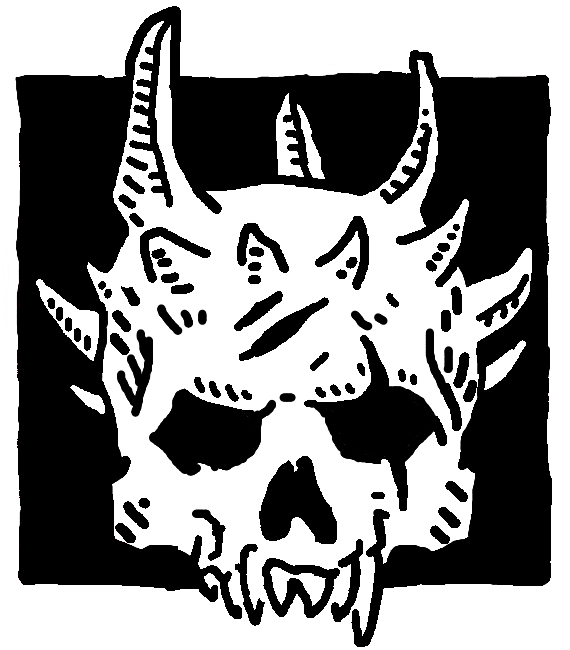
\includegraphics[width=2cm]{pics/wrath.png}

\noindent\textbf{\chosenofwrath}
\end{center}

La figurine gagne la règle \frenzy{}.

\columnbreak

\begin{center}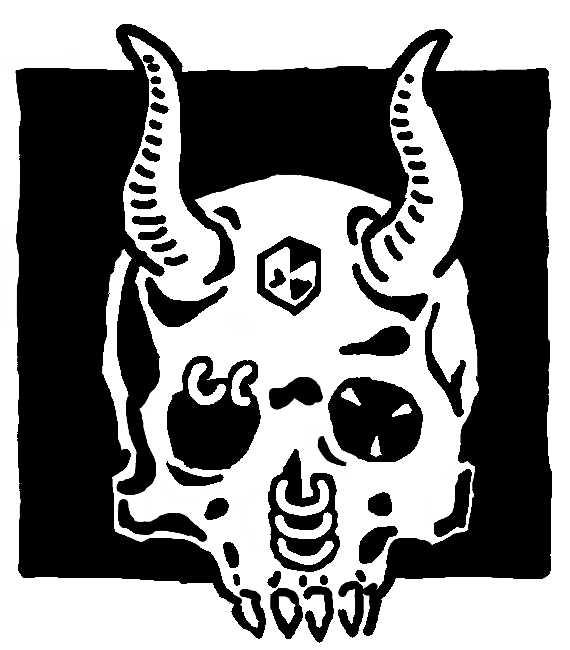
\includegraphics[width=2cm]{pics/lust.png}

\noindent\textbf{\chosenoflust}
\end{center}

L'unité gagne +2 en Mouvement et la règle \skirmisher{} mais ne peut pas prendre de figurines additionnelles, elle doit rester à la taille minimale.

\vspace*{0.2cm}\vspace*{\fill}

\begin{center}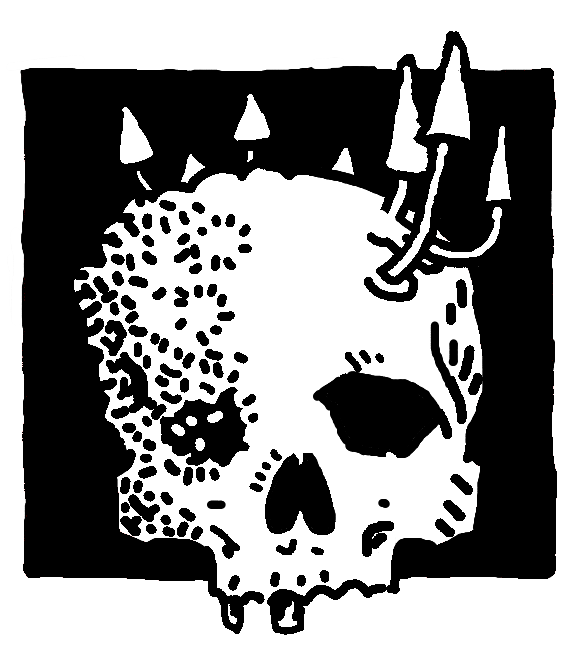
\includegraphics[width=2cm]{pics/pestilence.png}

\noindent\textbf{\chosenofpestilence}
\end{center}

La figurine gagne la règle \fear{}.

\end{multicols}

\armyspecialruleentry{\gazeofthegods}

La figurine ne peut pas refuser de Défi et doit en lancer un si aucune autre figurine ne le fait. Immédiatement après avoir tué un Monstre, ou un Personnage au cours d'un Défi, l'élément de figurine peut relancer tous ses jets pour toucher et pour blesser, et ce jusqu'à la fin de la prochaine Phase de Magie du joueur dont c'est le tour. Si deux figurines avec cette règle tuent un Monstre au même palier d'Initiative,  le propriétaire des figurines choisit laquelle des deux bénéficie du bonus.

\armyspecialruleentry{\lightningrage}

La figurine gagne une \wardsave{2} contre les attaques avec la règle \lightningattacks{}. Si elle est touchée par une de ces attaques, elle gagne la règle \frenzy{}.

\armyspecialruleentry{\inspiregreatness}

Si la figurine est de type Infanterie, toutes les figurines d'Infanterie de son unité peuvent effectuer une Attaque de Soutien supplémentaire depuis le deuxième rang (mais pas les rangs suivants).

\armyspecialruleentry{\survivalofthefittest}

Votre armée ne peut contenir au plus que deux figurines avec à la fois les règles \largetarget{} et \fly{}. Cette limite passe à 4 pour une Grande Armée, et à 1 pour une Patrouille.

\closearmyspecialrules







\newpage
\startarmyarmoury

\startitemlistonecol

\listitemonecol{\daemonweapon}Arme de Corps à Corps. Les attaques portées avec cette arme ont +1 en Force et la règle \magicalattacks{}.

\enditemlistonecol

\closearmyarmoury











\startarmynewsectionSP{\giftsofthedarkgods}

\spaceaftersection{}

Les \giftsofthedarkgods{} ont la règle \oneperarmy{}. Certains Dons sont réservés aux figurines dont l'allégeance va a un Dieu Sombre en particulier.

\begin{multicols}{2}\raggedcolumns

\startpricelistNSP

\pricelistitem{\beastbreaker}{70} Le porteur gagne la règle \terror{}. Si le porteur est le Général, la limite du nombre de figurines soumises à la règle \survivalofthefittest{} autorisées est augmentée de 1.

\pricelistitem{\daemonicwings}{50} Figurine à pied uniquement.

Le porteur gagne la règle \fly{8}.

\pricelistitem{\pathofthefallen}{45} Figurine d'Infanterie à pied uniquement.

Le porteur gagne +1 en Mouvement, +1 Point de Vie, -1 en Initiative, sa taille de socle passe à \unit{40x40}{\milli\meter} et son type de troupe devient \monstrousinfantry{}.

\pricelistitem{\thirdeyeofchange}{45\refsymbol{}/30}
\textbf{\dchange} uniquement.

\refsymbol{} Seul un \daemonprince{} doit payer \pts{45}, les autres figurines paient le deuxième prix.\newline
Le porteur augmente la valeur de sa \wardsave{} d'un point, jusqu'à obtenir 4+ au mieux.

\pricelistitem{\necroticmiasma}{40} \textbf{\pestilence} uniquement.

La figurine gagne la règle \breathweapon{\toxicattacks}. De plus, à chaque Manche de Corps à Corps, chaque figurine ennemie en contact socle à socle avec le porteur subit une touche de Force 1 avec la règle \armourpiercing{6} au palier d'Initiative 10.

\columnbreak
\pricelistitem{\wildlingblood}{40} Le porteur gagne la règle \inspiringpresence{}, qu'il soit le Général ou non. Cependant, seules les unités de type Bête de Guerre, Bête Monstrueuse, Infanterie Monstrueuse ou Monstre peuvent bénéficier de cette règle si le porteur n'est pas le Général.

Si le porteur est votre Général une unique unité de \wastelandtrolls{} de 6 figurines maximum peut être prise en choix d'Unité de Base.

Si le porteur est un Sorcier, il doit générer ses sorts dans la Discipline \wilderness{}, même s'il n'y a normalement pas accès ou devrait sélectionner une Discipline au hasard.

\pricelistitem{\wastehardenedskin}{30} Le porteur gagne la règle \innatedefence{6}, ou \innatedefence{5} si c'est une figurine d'\infantry{}. Ce Don ne peut pas être pris si le porteur monte une \manticore{}.

\pricelistitem{\hellishgrace}{25} \textbf{\lust} et à pied uniquement.

Si le porteur est une figurine d'\infantry{}, il gagne +2 en Mouvement. Sinon, il gagne la règle \swiftstride{}.

\pricelistitem{\soulreaper}{20} \textbf{\wrath} uniquement.

Si le porteur inflige au moins une blessure non sauvegardée avec une Attaque non Spéciale lors d'une Manche de Corps à Corps, lancez 1D6 à la fin de la phase. Sur un résultat de 4+, le porteur Récupère 1 Point de Vie. Ce Don peut être utilisé par une figurine avec un Profil Combiné, mais pas avec un Profil de Monstre Monté.

\endpricelistNSP

\end{multicols}

\closearmynewsection









\startarmymagicalitems

\armymagicalweapons

\startpricelist

\pricelistitem{\burningbladeofchaos}{65} Type : \hw{}. Les attaques portées avec cette arme ont les règles \flamingattacks{}, \multiplewounds{1D3}{} et \armourpiercing{6}. Après que toutes les attaques ont été résolues, pour chaque figurine tuée avec cette arme, l'unité de cette dernière subit une touche de Force 4 avec la règle \flamingattacks{}.

\pricelistitem{\spearofgagnir}{25} Type : \spear{}. Les attaques portées avec cette arme ont +1 en Force et la règle \lethalstrike{}.

\endpricelist

\armymagicalarmour

\startpricelist

\pricelistitem{\duelersshield}{10}Type : \shield{}. Au début de chaque Manche de Corps à Corps, désignez une figurine ennemie en contact socle à socle avec le porteur. Pour la durée de cette manche, un élément de cette figurine, de votre choix, subit un malus de -1 Attaque, jusqu'à un minimum de 1.

\endpricelist

\armyarcaneitems

\startpricelist

\pricelistitem{\daemonicidol}{35}
À chaque fois qu'une figurine ennemie effectue un jet sur la Table des Fiascos, vous pouvez augmenter ou réduire le résultat du jet de 1.

\endpricelist

\armymagicalbanners

\startpricelist

\pricelistitem{\ninetailedstandard}{50} \textbf{\infantry} uniquement.

Les unités alliées d'Infanterie sans la règle \skirmisher{} à moins de \distance{12} gagnent +1 en Mouvement.

\pricelistitem{\banneroftransmutation}{30} \textbf{\dchange} uniquement.

Les Attaques de Tir dirigées contre l'unité du porteur subissent un malus de -1 pour blesser.

\pricelistitem{\banneroffury}{25} \textbf{\wrath} uniquement.

Le porteur gagne la règle \frenzy{} et ne peut la perdre que si la bannière est capturée ou détruite. Les figurines de l'unité du porteur gagnent la règle \frenzy{} tant que le porteur l'a aussi et reste dans l'unité.

\pricelistitem{\banneroftemptation}{25} \textbf{\dlust} uniquement.

Une seule utilisation. La bannière peut être activée lorsque le porteur déclare une charge. La cible \textbf{doit} déclarer Tenir la Position en réaction à la charge, à moins qu'elle ne soit déjà en fuite. Cette unité peut déclarer d'autres réactions normalement si elle est chargée par d'autres unités par la suite.

\pricelistitem{\banneroffilth}{25} \textbf{\pestilence} uniquement.

Les Attaques de Corps à Corps de toutes les figurines de l'unité du porteur gagnent la règle \poisonedattacks{}.

\endpricelist

\closearmymagicalitems







%%% START OF THE ARMYLIST - Translators shouldn't have to edit it %%%


%%% v0.99.9

\armylist

\lordstitle

\showunit{
	name={\daemonprince},
	cost=245,
	profile={< 8 9 5 6 5 4 8 5 9},
	type=\monster{},
	basesize=50x50,
	unitsize={1},
	alliance={\daemonoftruechaos},
	alliancepic={truechaos},
	allianceoptions={introsentence=\mayreplacedaemonoftruechaoswith{}, change=20, lust=\free{}, pestilence=\free{}, wrath=\free{}},
	specialrules={\otherworldly{},\daemonicinstability{},\stubborn{},\daemonofadarkgod},
	options={
    	\magicalitemsallowance{}=\upto{}<25,
		\maytakeuptotwogifts{}=\unlimited{},
 		\magiclevelchoice{
			\magiclevel{1}=40,
			\magiclevel{2}=65,
			\magiclevel{3}=130,
			\magiclevel{4}=160,
		},
 		\platearmour{}=60,	
	},
	additional={%
		\def\tempunitrules{\unitrule{\daemonofadarkgod}{\daemonofadarkgodrule}}
		\vspace*{0.3cm}\unitrules{\tempunitrules}
	},		
}

\showunit{
	name={\lordofchaos},
	cost=160,
	profile={< 4 8 3 5 5 3 7 5 9},
	type=\infantry{},
	basesize=25x25,
	unitsize=1,
	alliance={\markoftruechaos},
	alliancepic={truechaos},
	allianceoptions={introsentence=\mayreplacemarkoftruechaoswith{}, change=30, lust=20, pestilence=40, wrath=30},
	specialrules={\inspiregreatness{},\gazeofthegods},
	armour={\platearmour},
	options={
		\magicalitemsallowance{}=\upto{}<100,	
	    \maytakeasinglegift{}=\unlimited{},
		\shield{}=5,
		\weapononechoice{
			\flail{}=10,
			\pw{}=10,
			\gw{}=15,
			\halberd{}=15,
			\lance{}=15,
		},
	},
	additional={%
		\def\tempmounts{
			\optionschoiceTWOCOL{}{
				\wastelandsteed{}=40,
				\hspace*{-0.3cm}\wastelandchariot{}=40,
				\hspace*{-0.3cm}\daemonicsteed{}=40,
				\hspace*{-0.3cm}\manticore{}=120,
				\hspace*{-0.3cm}\wastelanddragon{}=270,
				\columnbreak\pestilentpalanquin{}=15,
				\crusher{}=40,
				\steedoflust{}=40,
				\discofchange{}=60,
			},
		}
		\vspace*{0.2cm}\mounts{\tempmounts}
	},
}

\showunit{
	name={\sorcererlord},
	cost=200,
	profile={< 4 5 3 4 4 3 5 3 8},
	type=\infantry{},
	basesize=25x25,
	unitsize=1,
	alliance={\markoftruechaos},
	alliancepic={truechaos},
	allianceoptions={introsentence=\mayreplacemarkoftruechaoswith{}, change=40, lust=10, pestilence=15},
	armour={\platearmour},
	specialrules={\gazeofthegods},
	magiclevel=3,
	magicpaths={\pathdependingonthemodelsmark},
	options={
		\magicalitemsallowance{}=\upto{}<100,
	    \maytakeasinglegift{}=\unlimited{},
		\magiclevel{4}=30,
	},
	additional={%
		\def\tempmounts{
			\optionschoiceTWOCOL{}{
				\wastelandsteed{}=35,
				\hspace*{-0.3cm}\wastelandchariot{}=40,
				\hspace*{-0.3cm}\daemonicsteed{}=60,
				\hspace*{-0.3cm}\manticore{}=120,
				\hspace*{-0.3cm}\wastelanddragon{}=320,
				\columnbreak\pestilentpalanquin{}=15,
				\steedoflust{}=30,
				\discofchange{}=50,
			},
		}
		\mounts{\tempmounts}
	},
}







\heroestitle

\showunit{
	name={\sorcerer},
	profile={< 4 5 3 4 4 2 4 2 8},
	type=\infantry{},
	basesize=25x25,
	unitsize=1,
	armour={\platearmour},
	specialrules={\gazeofthegods},			
	additional={%
		\vspace*{-0.1cm}\begin{center}\mustbecomeoneofthefollowingNOC{}\end{center}
		\setlength{\columnsep}{1cm}
		\setlength{\columnseprule}{0.5pt}
		\renewcommand{\columnseprulecolor}{\color{black!30}}

		\vspace*{-0.2cm}\begin{multicols}{2}\raggedcolumns

		\begin{center}\Largefontsize{\antiquefont\sorcerer{} (\pts{90})}\end{center}%	

		\def\tempalliance{\markoftruechaos}
		\def\tempalliancepic{truechaos}
		\def\tempallianceoptions{introsentence=\mayreplacemarkoftruechaoswith{}, change=25, lust=10, pestilence=15}
		\def\tempmagiclvl{1}
		\def\tempmagicpaths{\pathdependingonthemodelsmark}

		\vspace*{-0.3cm}{\setlength{\parskip}{0.3cm}
		\noindent\parbox{\columnwidth}{\begin{minipage}[c][][b]{0.045\textwidth}%
			\includegraphics[width=\textwidth]{pics/\tempalliancepic.png}%
		\end{minipage}%
		\hspace*{0.15cm}\begin{minipage}[c]{0.40\textwidth}%
			\alliance{\tempalliance}%
		\end{minipage}\vspace*{-0.1cm}}
		
		\noindent\parbox{\columnwidth}{\expandafter\allianceoptions\expandafter{\tempallianceoptions}}
		
		\magic{\tempmagiclvl}{\tempmagicpaths}
		}

		\def\tempmounts{
			\steedoflust{}=20,
			\wastelandsteed{}=25,
			\pestilentpalanquin{}=30,
			\wastelandchariot{}=50,
			\discofchange{}=50,
			\daemonicsteed{}=60,
		}
		
		\def\tempoptions{
			\magicalitemsallowance{}=\upto{}<50,			
	 	   \maytakeasinglegift{}=\unlimited{},
			\magiclevel{2}=25,
		}
		
		\vspace*{0.2cm}
		\mounts{\tempmounts}
		\options{\tempoptions}

		\vspace*{\fill}\columnbreak
		
		\begin{center}\Largefontsize{\antiquefont\wrathpriest{} (\pts{100})}\end{center}

		\def\tempalliance{\markofwrath}
		\def\tempalliancepic{wrath}
		\def\tempspecialrules{\inspiregreatness{},\magicresistance{2},\wordsofscorn}
		\def\tempunitrules{\unitrule{\wordsofscorn}{\wordsofscornrule}}
		\def\tempmounts{
			\wastelandsteed{}=25,
			\crusher{}=30,
			\wastelandchariot{}=50,
			\daemonicsteed{}=60,
		}
		\def\tempoptions{
			\magicalitemsallowance{}=\upto{}<50,		
	 	   \maytakeasinglegift{}=\unlimited{},
			\weapononechoice{
				\flail{}=5,
				\gw{}=10,
			},		
		}

		\vspace*{-0.3cm}{\setlength{\parskip}{0.3cm}
		\noindent\begin{minipage}[c][][b]{0.045\textwidth}%
			\includegraphics[width=\textwidth]{pics/\tempalliancepic.png}%
		\end{minipage}%
		\hspace*{0.15cm}\begin{minipage}[c]{0.40\textwidth}%
			\alliance{\tempalliance}%
		\end{minipage}\vspace*{-0.1cm}%
		
		\noindent\specialrules{\tempspecialrules}
		}
		
		\vspace*{0.2cm}\unitrules{\tempunitrules}
		
		\mounts{\tempmounts}
		
		\options{\tempoptions}
		\vspace*{\fill}\end{multicols}
		\setlength{\columnseprule}{0pt}
	},
}

\showunit{
	name={\harbingerofchaos},
	cost=100,
	profile={< 4 7 3 5 4 2 6 4 8},
	type=\infantry{},
	basesize=25x25,
	unitsize=1,
	alliance={\markoftruechaos},
	alliancepic={truechaos},
	allianceoptions={introsentence=\mayreplacemarkoftruechaoswith{}, change=20, lust=10, pestilence=30, wrath=20},
	armour={\platearmour},
	specialrules={\inspiregreatness{}, \gazeofthegods},	
	options={
		\magicalitemsallowance{}=\upto{}<50,
		\bsb{}=25,
	    \maytakeasinglegift{}=\unlimited{},
		\shield{}=5,
		\weapononechoice{
			\flail{}=5,
			\pw{}=5,
			\gw{}=10,
			\halberd{}=10,
			\lance{}=15,
		},
	},
	additional={%
		\def\tempmounts{
			\optionschoiceTWOCOL{}{
				\wastelandsteed{}=30,
				\hspace*{-0.3cm}\wastelandchariot{}=50,
				\hspace*{-0.3cm}\daemonicsteed{}=60,
				\hspace*{-0.3cm}\manticore{}=155,
				\pestilentpalanquin{}=30,
				\crusher{}=35,
				\steedoflust{}=35,
				\discofchange{}=50,
			},
		}
		\vspace*{0.2cm}\mounts{\tempmounts}
	},
}

\showunit{
	name={\barbarianchief},
	cost=45,
	profile={< 4 5 4 4 4 2 5 3 8},
	type=\infantry{},
	basesize=25x25,
	unitsize=1,
	alliance={\markoftruechaos},
	alliancepic={truechaos},
	allianceoptions={introsentence=\mayreplacemarkoftruechaoswith{}, change=5, lust=5, pestilence=15, wrath=10},
	armour={\la},
	specialrules={\inspirebarbarians},
	options={
		\magicalitemsallowance{}=\upto{}<50,
		\bsb{}\refsymbol{}=25,
		\hspace*{0.3cm}\refsymbol{} \onlyifanotherBCisthegeneral{}=,
		\maytakeasinglegiftbarbarian{}=\unlimited{},
		\shield{}=4,
		\ha{}=5,
		\throwingweapons{}=3,
		\weapononechoice{
			\flail{}=3,
			\spear{}=3,
			\lightlance{}=3,
			\pw{}=3,
			\gw{}=4,
		},
	},	
	mounts={
		\warhorse{}=20,
	},
	additional={%
		\def\tempunitrules{\unitrule{\inspirebarbarians}{\inspirebarbariansrule}}
		\vspace*{0.1cm}\unitrules{\tempunitrules}
		
		\begin{center}\maytakeoneofthefollowingrules{}\spacebeforecolon{}:\end{center}
		\setlength{\columnseprule}{0.5pt}
		\setlength{\columnsep}{1cm}
		\renewcommand{\columnseprulecolor}{\color{black!30}}
		\vspace*{-0.1cm}\begin{multicols}{2}\raggedcolumns
		
		\begin{center}\Largefontsize\antiquefont\osklanderjarl{} (\pts{40})
		
		\oneofakind{}, \only{\infantry}\end{center}
		
		\noindent\osklanderjarlrule{}
		
		\vspace*{\fill}\columnbreak
		
		\begin{center}\Largefontsize\antiquefont\makharkhan{} (\pts{30})
		
		\oneofakind{}\end{center}
		
		\noindent\makharkhanrule{}
		
		\vspace*{\fill}\end{multicols}
		\setlength{\columnseprule}{0pt}
	},	
}










\newpage
\toctarget{mountstitle}{\mountstitle}

\showunit{
	name={\warhorse},
	profile={< 8 3 - 3 3 1 3 1 5},
	type=\warbeast{},
	basesize=25x50,
	specialrules={\fastcavalry},
	armour={\mountsprotection{6}},
	additional={%
		\def\tempoptions{\mayexchangefastcavformountsprotectionLONG{}=10,}
		\vspace*{0.15cm}\options{\tempoptions}
	},
}

\showunit{
	name={\wastelandsteed},
	QRSname={\wastelandsteedSHORT},
	profile={< 8 3 - 4 3 1 3 1 5},
	type=\warbeast{},
	basesize=25x50,
	armour={\mountsprotection{6},\barding},
}

\showunit{
	name={\daemonicsteed},
	profile={< 8 4 - 5 5 3 2 2 8},
	type=\monstrousbeast{},
	basesize=50x50,
	specialrules={\magicalattacks{},\fear},
	armour={\mountsprotection{6}},
	options={\barding{}=10,},
}

\showunit{
	notinQRS=yes,
	name={\wastelandchariot},
	profile={\chariot{}< - - - 5 5 4 - - -,
			 \crew{} (1)< - 5 3 4 - - 4 2 8,
			 \wastesteed{} (2)< 8 3 - 4 - - 3 1 -,
			 },
	type=\chariot{},
	basesize=50x100,
	alliance={\samemarkasthecharacter{} \textnormal{\only{\crew}}},
	specialrules={\impacthits{+1}},
	weapons={\halberd{} \only{\crew}},
	armour={\mountsprotection{6}},
	options={
		\wastelandraider{} \only{\general}=\permodel{}<20,
		\barding{}=20,
	},
	unitrules={\unitrule{\wastelandraider}{\wastelandraiderrule}},
}

\showunit{
	name={\manticore},
	profile={< 6 5 - 5 5 4 5 3 5},
	type=\monstrousbeast{},
	basesize=50x100,
	unitsize=SPECIAL-{\textbf{(\survivalofthefittest{})}},
	additional={%
		\def\tempspecialrules{\multiplewounds{1D3}{},\lethalstrike{},\frenzy{},\largetarget{},\fear{},\fly{8}}
		\vspace*{-0.2cm}\specialrules{\tempspecialrules}
	},
}

\showunit{
	name={\wastelanddragon},
	QRSname={\wastelanddragonSHORT},
	profile={< 6 5 1 6 6 6 3 6 9},
	type=\monster{},
	basesize=50x100,
	unitsize=SPECIAL-{\textbf{(\oneofakind{}, \survivalofthefittest{})}},
	armour={\innatedefence{3}},	
	additional={%
		\def\tempspecialrules{\breathweapon{\Strength{} 4, \flamingattacks}, \breathweapon{\Strength{} 3, \armourpiercing{3}},\fly{7}}
		\vspace*{0.3cm}\specialrules{\tempspecialrules}
	}
}

\newpage
\showunit{
	name={\discofchange},
	profile={< 1 3 - 4 4 1 4 3 7},
	type=\warbeast{},
	basesize=50x50,
	unitsize=SPECIAL-{\textbf{\only{\markofchange}}},
	alliance={\markofchange},
	alliancepic={change},
	specialrules={\magicalattacks{},\fly{8}},
	armour={\mountsprotection{6}},
}

\showunit{
	name={\crusher},
	profile={< 7 5 - 5 4 3 2 3 7},
	type=\monstrousbeast{},
	basesize=50x75,
	unitsize=SPECIAL-{\textbf{\only{\markofwrath}}},
	alliance={\markofwrath},
	alliancepic={wrath},
	specialrules={\magicalattacks{},\fear},
	armour={\mountsprotection{6}},
}

\showunit{
	name={\steedoflust},
	profile={< 10 3 - 3 3 1 5 1 8},
	type=\warbeast{},
	basesize=25x50,
	unitsize=SPECIAL-{\textbf{\only{\markoflust}}},
	alliance={\markoflust},
	alliancepic={lust},
	specialrules={\poisonedattacks{},\magicalattacks{},\vanguard},
	armour={\mountsprotection{6}},
}

\showunit{
	name={\pestilentpalanquin},
	profile={< 4 3 3 3 3 3 3 6 7},
	type=\infantry{},
	basesize=50x50,
	unitsize=SPECIAL-{\textbf{\only{\markofpestilence}}},
	alliance={\markofpestilence},
	alliancepic={pestilence},
	specialrules={\poisonedattacks{},\magicalattacks},
	armour={\mountsprotection{6}},
}










\coreunitstitle

\showunit{
	name={\wastelandwarriors},
	QRSname={\wastelandwarrior},
	cost=110,
	profile={< 4 5 3 4 4 1 4 2 8},
	type=\infantry{},
	unitsize=10,
	costpermodel=13,
	maxmodels=30,
	basesize=25x25,
	alliance={\markoftruechaos},
	alliancepic={truechaos},
	allianceoptions={introsentence=\mayreplacemarkoftruechaoswith{} \Xmodelsorless{25}, change=\permodel{}<1, lust=\permodel{}<1, pestilence=\permodel{}<3, wrath=\permodel{}<2},
	armour={\platearmour{},\shield},
	options={
		\weapononechoice{
			\pw{}=\permodel{}<1,
			\gw{}=\permodel{}<2,
			\halberd{}=\permodel{}< 3
		},
	},
    commandgroup={champion=10,  musician=10, banner=10, veteranstandardbearer=yessir},
}

\showunit{
	name={\fallen},
	QRSname={\fallenSING},
	cost=85,
	profile={< 6 4 - 4 4 1 4 \starsymbol{} 8},
	type=\infantry{},
	unitsize=5,
	costpermodel=15,
	maxmodels=12,
	basesize=25x25,
	alliance={\markoftruechaos},
	alliancepic={truechaos},
	allianceoptions={introsentence=\mayreplacemarkoftruechaoswith{}, change=\permodel{}<1, lust=\permodel{}<1, pestilence=\permodel{}<3, wrath=\permodel{}<2},
	specialrules={\randomattacks{1D3},\frenzy{},\immunetopsychology{},\skirmisher},
	armour={\platearmour},
	commandgroup={champion=10},
}

\showunit{
	name={\warhounds},
	QRSname={\warhound},
	cost=45,
	profile={< 7 4 - 3 3 1 3 1 5},
	type=\warbeast{},
	unitsize=5,
	maxmodels=35,
	costpermodel=4,
	basesize=25x50,
	specialrules={\poisonedattacks{},\vanguard{},\insignificant},
	options={
		\innatedefence{5}=\permodel{}<2,
	},
}

\showunit{
	name={\barbarians},
	QRSname={\barbarian},
	cost=70,
	profile={< 4 4 3 3 3 1 3 1 7},
	type=\infantry{},
	unitsize=20,
	maxmodels=50,
	costpermodel=5,
	basesize=25x25,
	alliance={\markoftruechaos},
	alliancepic={truechaos},
	allianceoptions={introsentence=\mayreplacemarkoftruechaoswith{}, change=\permodel{}<1, lust=\permodel{}<1, pestilence=\permodel{}<2, wrath=\permodel{}<1},
	armour={\la},
	options={
		\throwingweapons{}=\permodel{}<1,
		\onechoiceonly{
			\pw{}=\free{},
			\shield{}=\permodel{}<1,
			\spear{} \wordand{} \shield{}=\permodel{}<1,
			\flail{}=\permodel{}<2,
			\gw{}=\permodel{}<3,
		},
	},
	commandgroup={champion=10, banner=10, veteranstandardbearer=yessir, musician=10},
}

\showunit{
	name={\barbarianhorsemen},
	QRSname={\barbarianhorseman},
	cost=75,
	profile={\rider{}< 4 4 3 3 3 1 3 1 7,
			 \warhorse{}< 8 3 - 3 3 1 3 1 5
	},
	type=\cavalry{},
	unitsize=5,
	maxmodels=15,
	costpermodel=11,
	basesize=25x50,
	alliance={\markoftruechaos{} \textnormal{\only{\rider}}},
	alliancepic={truechaos},
	allianceoptions={introsentence=\mayreplacemarkoftruechaoswith{}, change=\permodel{}<1, lust=\permodel{}<2, pestilence=\permodel{}<2, wrath=\permodel{}<2},
	specialrules={\fastcavalry},
	armour={\la{},\mountsprotection{6}},
	options={
		\mayexchangefastcavformountsprotection{}=\permodel{}<1,
		\shield{}=\permodel{}<1,
		\throwingweapons{}=\permodel{}<2,
		\weapononechoice{
			\flail{}=\permodel{}<1,
			\lightlance{}=\permodel{}<1,
		},
	},
	commandgroup={champion=10, banner=10, veteranstandardbearer=yessir, musician=10},
}









\specialunitstitle

\showunit{
	name={\wastelandchariot},
	QRSname={\wastelandchariot{}\refsymbol},
	profile={\chariot{}< - - - 5 5 - - - -,
			 \crew{} (2)< - 5 3 4 - - 4 2 8,
			 [\wastesteed{} (2)]< 8 3 - 4 - 4 3 1 5,
			 [\mauler{} (1)]< 6 4 - 5 - 6 2 3 6,
	},
	type=\chariot{},
	unitsize=1,
	basesize=50x100,
	alliance={\markoftruechaos{} \textnormal{\only{\crew}}},
	alliancepic={truechaos},
	allianceoptions={introsentence=\mayreplacemarkoftruechaoswith{}, change=10, lust=20, pestilence=20, wrath=10},
	specialrules={\impacthits{+1}},
	weapons={\halberd{} \only{\crew}},
	additional={%
		\begin{center}\musttakeoneofthefollowingNOC{}\end{center}
		\setlength{\columnseprule}{0.5pt}
		\setlength{\columnsep}{1cm}
		\renewcommand{\columnseprulecolor}{\color{black!30}}
		\vspace*{-0.2cm}\begin{multicols}{2}\raggedcolumns
		
		\begin{center}\Largefontsize\antiquefont\pairofwastesteeds{} (\pts{95})\end{center}
		
		\def\temparmour{\platearmour}
		\armour{\temparmour}
		
		\vspace*{\fill}\columnbreak
		
		\begin{center}\Largefontsize\antiquefont\mauler{} (\pts{140})\end{center}
		
		\def\temparmour{\platearmour{},\mountsprotection{6}}
		\armour{\temparmour}
		
		\def\tempspecialrules{\fear{},\grindingattacks{1D3} \only{\mauler}}
		\vspace*{0.3cm}\specialrules{\tempspecialrules}
		
		\def\tempoptions{\mountsprotection{5}=15,}
		\vspace*{0.2cm}\options{\tempoptions}
		
		\vspace*{\fill}\end{multicols}
		\setlength{\columnseprule}{0pt}
	},
}

\showunit{
	name={\wastelandknights},
	QRSname={\wastelandknight},
	cost=170,	
	profile={\rider{}< 4 5 3 4 4 1 5 2 8,
					\wastesteed{}< 8 3 - 4 3 1 3 1 5},
	type=\cavalry{},
	unitsize=5,
	maxmodels=10,
	costpermodel=32,
	basesize=25x50,
	alliance={\markoftruechaos{} \textnormal{\only{\rider}}},
	alliancepic={truechaos},
	allianceoptions={introsentence=\mayreplacemarkoftruechaoswith{}, change=\permodel{}<2, lust=\permodel{}<3, pestilence=\permodel{}<4, wrath=\permodel{}<3},
	specialrules={\fear},
	armour={\platearmour{},\shield{},\barding{},\mountsprotection{6}},
	weapons={\lance{} \only{\rider}},
	options={
		\mayreplacelancewithdaemonweapon{}=\permodel{}<4,
	},
	commandgroup={champion=10, banner=10, bannerallowance=50, musician=10},
}

\showunit{
	name={\chosen},
	QRSname={\chosenSING},
	cost=120,
	profile={< 4 6 3 4 4 1 5 2 8},
	type=\infantry{},
	unitsize=10,
	maxmodels=25,
	costpermodel=12,
	basesize=25x25,
	alliance={\markoftruechaos},
	alliancepic={truechaos},
	allianceoptions={introsentence=\mayreplacemarkoftruechaoswith{}, change=\permodel{}<2, lust=40, pestilence=\permodel{}<4, wrath=\permodel{}<3},
	specialrules={\immunetopsychology{},\chosenofthegods},
	armour={\platearmour{},\shield},
	options={
		\weapononechoice{
			\pw{}=\permodel{}<1,
			\gw{}=\permodel{}<2,
			\halberd{}=\permodel{}<3,
		},
	},
	commandgroup={champion=10 [80], chosenofchangeopt=[\chosenofchange], championallowance=25, banner=10, bannerallowance=50, musician=10},
}

\showunit{
	name={\oncechosen},
	QRSname={\oncechosenSING},
	cost=100,
	profile={< 5 5 3 4 4 3 4 3 8},
	type=\monstrousinfantry{},
	unitsize=3,
	maxmodels=9,
	costpermodel=30,
	basesize=40x40,
	alliance={\markoftruechaos},
	alliancepic={truechaos},
	allianceoptions={introsentence=\mayreplacemarkoftruechaoswith{}, change=\permodel{}<4, lust=50, pestilence=\permodel{}<8, wrath=\permodel{}<6},
	specialrules={\chosenofthegods},
	armour={\platearmour},
	options={
		\shield{}=\permodel{}<3,
		\weapononechoice{
			\pw{}=\permodel{}<3,
			\flail{}=\permodel{}<5,
			\gw{}=\permodel{}<7,
			\halberd{}=\permodel{}<7,
		},
	},
	commandgroup={champion=10 [70], chosenofchangeopt=[\chosenofchange], championallowance=25, banner=10, bannerallowance=25, musician=10},
}

\showunit{
	name={\hellriders},
	QRSname={\hellrider},
	cost=75,
	profile={\rider{}< 4 4 4 3 3 1 5 1 7,
					\steedoflust{}< 10 3 - 3 3 1 5 1 7,
	},
	type=\cavalry{},
	unitsize=5,
	maxmodels=15,
	costpermodel=10,
	basesize=25x50,
	alliance={\markoflust},
	alliancepic={lust},
	armour={\shield{},\mountsprotection{6}},
	weapons={\lightlance{},\hellishwhip},
	commandgroup={champion=10, banner=10, musician=10},
	additional={%
		\def\tempspecialrules{\poisonedattacks{} \only{\steed},\fastcavalry{},\lightningreflexes{} \only{\rider}, \magicalattacks{} \only{\steed}}
		\specialrules{\tempspecialrules}
		
		\def\tempunitequipment{\equipmentdef{\hellishwhip}{\hellishwhiprule}}
		\vspace*{0.1cm}\unitequipment{\tempunitequipment}
	},
}

\showunit{
	name={\wastelandtrolls},
	QRSname={\wastelandtroll},
	cost=100,
	profile={< 6 3 1 5 4 3 1 3 4},
	type=\monstrousinfantry{},
	unitsize=3,
	maxmodels=10,
	costpermodel=42,
	basesize=40x40,
	specialrules={\trollbelch{},\fear{},\regeneration{4},\stupidity},
	unitrules={\unitrule{\trollbelch}{\trollbelchrule}},
	options={
		\markofpestilence{}=\permodel{}<6,
		 \pw{}=\permodel{}<3,
	},
}

\showunit{
	name={\dragoncentaurs},
	QRSname={\dragoncentaur},
	cost=205,
	profile={< 7 4 2 5 5 4 2 3 8},
	type=\monstrousbeast{},
	unitsize=3,
	maxmodels=5,
	costpermodel=68,
	basesize=50x75,
	alliance={\markoftruechaos},
	alliancepic={truechaos},
	specialrules={\stomp{2},\lightningrage},
	armour={\la{},\innatedefence{5}},
	options={
		\weapononechoice{
			\pw{}=\permodel{}<3,
			\halberd{}=\permodel{}<6,
			\gw{}=\permodel{}<10,
		},
	},
	commandgroup={champion=10, banner=10, musician=10},
}

\showunit{
	name={\fallenbeast},
	cost=65,
	profile={< \starsymbol{} 3 - 4 5 3 2 \starsymbol{} 10},
	type=\monstrousbeast{},
	unitsize=1,
	basesize=40x40,
	alliance={\markoftruechaos},
	alliancepic={truechaos},
	allianceoptions={introsentence=\mayreplacemarkoftruechaoswith{}, change=5, lust=15, pestilence=10, wrath=5},
	additional={%
		\def\tempspecialrules{\randomattacks{1D6+1},\unbreakable{},\randommovement{3D6},\fear{},\wastelandwanderer}
		\vspace*{0.2cm}\specialrules{\tempspecialrules}
		
		\def\tempunitrules{\unitrule{\wastelandwanderer}{\wastelandwandererrule}}
		\vspace*{0.2cm}\unitrules{\tempunitrules}
	},
}

\showunit{
	name={\bloodbeast},
	cost=175,
	profile={< 7 3 - 6 5 5 3 5 4},
	type=\monster{},
	unitsize=1,
	basesize=50x100,
	specialrules={\frenzy{},\hatred{},\ritesofbinding},
	armour={\innatedefence{4}},	
	additional={%
		\def\tempunitrules{\unitrule{\ritesofbinding}{\ritesofbindingrule}}
		\vspace*{0.2cm}\unitrules{\tempunitrules}
	},
}









\rareunitstitle

\showunit{
	name={\crusherknights},
	QRSname={\crusherknight},
	cost=170,
	profile={\rider{}< 4 5 3 4 4 1 5 2 8,
			 		\crusher{}< 7 5 - 5 4 3 2 3 7},
	type=\monstrouscavalry{},
	unitsize=2,
	maxmodels=5,
	costpermodel=55,
	basesize=50x75,
	alliance={\markofwrath},
	alliancepic={wrath},
	specialrules={\magicalattacks{} \only{\crusher},\chosenofthegods{} \only{\rider},\fear},
	armour={\platearmour{},\shield{},\mountsprotection{6}},
	options={
		\weapononechoice{
			\lance{}=\permodel{}<2,
			\daemonweapon{}=\permodel{}<6,
		},
	},
	commandgroup={champion=10, banner=10, bannerallowance=50, musician=10},
}

\showunit{
	name={\hellscreamcannon},
	cost=190,
	profile={< 4 4 3 5 6 5 1 4 7},
	type=\monster{},
	unitsize=1,
	basesize=100x150,
	specialrules={\otherworldly{},\frenzy{},\daemonicinstability{},\stubborn},
	weapons={\hellscreamcannon},
	armour={\innatedefence{5}},	
	additional={%
		\def\tempunitequipment{\equipmentdef{\hellscreamcannon}{\hellscreamcannonrule}}
		\vspace*{0.2cm}\unitequipment{\tempunitequipment}
	}
}

\showunit{
	name={\battleshrine},
	cost=130,
	profile={\shrinepriest{} (1)< - 5 3 4 - - 4 2 8,
			 		\shrinebearers{}< 5 3 - 4 5 5 2 \starsymbol{} 7},
	type=\monstrousinfantry{},
	unitsize=1,
	basesize=50x100,
	alliance={\markoftruechaos},
	alliancepic={truechaos},
	allianceoptions={introsentence=\mayreplacemarkoftruechaoswith{}, change=10, lust=10, pestilence=10, wrath=10},
	armour={\mountsprotection{6},\ha},
	additional={%
		\def\tempspecialrules{\randomattacks{3D3} \only{\shrinebearers},\largetarget{},\thedarkgodsarewatching{},\fear{},\wardsave{4}}
		\vspace*{0.2cm}\specialrules{\tempspecialrules}
		
		\def\tempunitrules{\unitrule{\thedarkgodsarewatching}{\thedarkgodsarewatchingrule}}
		\vspace*{0.2cm}\unitrules{\tempunitrules}
	},
}

\showunit{
	name={\chimera},
	cost=200,
	profile={< 6 4 - 6 5 4 3 7 5},
	type=\monster{},
	unitsize=SPECIAL-{\textbf{(\survivalofthefittest{})} \labels@Singlemodel{}},
	basesize=50x100,
	specialrules={\regeneration{5},\fly{8}},
	armour={\innatedefence{4}},	
	options={
		\breathweapon{\Strength{} 4, \flamingattacks}=30,
	},
}

\showunit{
	name={\vortexfiend},
	cost=175,
	profile={< 6 4 - 5 5 5 3 \starsymbol{} 8},
	type=\monster{},
	unitsize=1,
	basesize=50x100,
	alliance={\markofchange},
	alliancepic={change},
	armour={\innatedefence{5}},	
	additional={%
		\def\tempspecialrules{\randomattacks{1D6+2},\hardtarget{},\channel{},\wardsave{5},\wavesofchange}
		\vspace*{0.3cm}\specialrules{\tempspecialrules}
		
		\def\tempunitrules{\unitrule{\wavesofchange}{\wavesofchangerule}}
		\vspace*{0.2cm}\unitrules{\tempunitrules}
	},
}

\showunit{
	name={\elderdragoncentaur},
	cost=230,
	profile={< 7 6 3 6 6 6 4 5 9},
	type=\monster{},
	unitsize=1,
	basesize=50x75,
	specialrules={\immunetopsychology{},\lightningrage{},\swiftstride},
	armour={\innatedefence{4}},	
	options={
		\la{}=20,
		\weapononechoice{
			\gw{}=20,
			\halberd{}=20,
			\pw{}=20,
		},
	},
}

\showunit{
	name={\wastelandgiant},
	cost=140,
	profile={< 6 3 - 6 5 6 3 \starsymbol{} 10},
	type=\monster{},
	basesize=50x75,
	unitsize=1,
	alliance={\markoftruechaos},
	alliancepic={truechaos},
	allianceoptions={introsentence=\mayreplacemarkoftruechaoswith{}, change=30, lust=60, pestilence=10, wrath=\free},
	specialrules={\immunetopsychology{},\stubborn{},\giantattacks{},\chosenofthegods},
	commandgroup={champion=90, championrestriction=\markofchange},
	additional={%
		\def\tempunitrules{%
			\unitrule{\giantattacks}{\giantattacksrule}
			\unitrule{\bellow}{\bellowrule}
			\unitrule{\jump}{\jumprule}
			\unitrule{\grab}{\grabrule}
			\unitrule{\swing}{\swingrule}
			\unitrule{\thump}{\thumprule}
			\unitrule{\smashname}{\smashrule}
		}
		\vspace*{0.3cm}\unitrules{\tempunitrules}
		\giantattackstable
	},
}


%%% Quick Reference Sheet - AB_qrs.tex is automatic and shouldn't be edited %%%

\quickrefsheettitle

% Script to automatically draw the Quick Ref Sheet

\renewcommand{\arraystretch}{1.2}

\providebool{QRSbool}

\providebool{whiterow}

\newcommand{\QRSrowcolor}{\ifbool{whiterow}{\global\boolfalse{whiterow}}{\rowcolor{black!10}\global\booltrue{whiterow}}}

\newcommand{\QRSstarttab}[1]{%
	\noindent%
	\setlength{\tabcolsep}{2pt}%
	\begin{tabular}{@{}cp{3.2cm}M{\profilecellsize}@{}M{\profilecellsize}@{}M{\profilecellsize}@{}M{\profilecellsize}@{}M{\profilecellsize}@{}M{\profilecellsize}@{}M{\profilecellsize}@{}M{\profilecellsize}@{}M{\profilecellsize}}%

	& \antiquefont\large{\textbf{#1}} & \textbf{\labels@M} & \textbf{\labels@WS} & \textbf{\labels@BS} & \textbf{\labels@S} & \textbf{\labels@T} & \textbf{\labels@W} & \textbf{\labels@I} & \textbf{\labels@A} & \textbf{\labels@Ld}%
}%

\newcommand{\QRSclosetab}{\end{tabular}\bigskip}%

\newcommand{\QRSprintline}[4]{%
	\tabularnewline%
	\ifnumequal{\rowmulti}{1}{\QRSrowcolor}{}%
	\DTLifeq*{\rowcategory}{\labels@lords}{\antiquefont\bfseries \labels@lordsInitial}{}%
	\DTLifeq*{\rowcategory}{\labels@heroes}{\antiquefont\bfseries \labels@heroesInitial}{}%
	\DTLifeq*{\rowcategory}{\labels@coreunits}{\antiquefont\bfseries \labels@coreunitsInitial}{}%
	\DTLifeq*{\rowcategory}{\labels@specialunits}{\antiquefont\bfseries \labels@specialunitsInitial}{}%
	\DTLifeq*{\rowcategory}{\labels@rareunits}{\antiquefont\bfseries \labels@rareunitsInitial}{}%
	\DTLifeq*{\rowcategory}{\labels@mounts}{\antiquefont\bfseries \labels@mountsInitial}{}%
	&%
	\ifnumequal{\rowmulti}{1}{%no Multiprofile
		\rowname%
		\expandafter\parselist\expandafter{\rowprofile}{\locallists@profileslist}%
		\forlistloop{\QRSmonoprofile}{\locallists@profileslist}%
	}{% Multiprofile
		\rowname &&&&&&&&&%
		\expandafter\parselist\expandafter{\rowprofile}{\locallists@profileslist}%
		\forlistloop{\QRSmultiprofile}{\locallists@profileslist}%
	}%
}

\newcommand{\QRSmultiprofile}[1]{%
	\tabularnewline%
	\QRSrowcolor{}&%
	\splitatinf{#1}\local@unitname\local@unitprofile%
	- \local@unitname \expandafter\caraclist\expandafter{\local@unitprofile}%
}%

\newcommand{\QRSmonoprofile}[1]{%
	\splitatinf{#1}\local@unitname\local@unitprofile%
	\expandafter\caraclist\expandafter{\local@unitprofile}%
}%

\newcommand{\QRSprinttab}[1]{%
	\global\booltrue{whiterow}%
	\DTLforeach*[#1]%
	{profiles}{\rowname=name, \rowtrooptype=trooptype, \rowcategory=category, \rowprofile=profile, \rowmulti=multipleprofile}{%
      		\QRSprintline{\rowname}{\rowcategory}{\rowprofile}{\rowmulti}%
	}%
}%

\providebool{QRSisempty}
\global\boolfalse{QRSisempty}%

\newcommand{\QRScheckifempty}[1]{%
	\global\booltrue{QRSisempty}%
	\DTLforeach*[#1]%
	{profiles}{\rowname=name, \rowtrooptype=trooptype, \rowcategory=category, \rowprofile=profile, \rowmulti=multipleprofile}{%
		\global\boolfalse{QRSisempty}\dtlbreak%
	}%
}%

\newcommand{\QRSifnotempty}[1]{%
	\ifbool{QRSisempty}{}{#1}%
}%

\begin{center}
{\antiquefont\bfseries \labels@lordsInitial}\spacebeforecolon{}: \labels@lords{} - %
{\antiquefont\bfseries \labels@heroesInitial}\spacebeforecolon{}: \labels@heroes{} - %
{\antiquefont\bfseries \labels@coreunitsInitial}\spacebeforecolon{}: \labels@coreunits{} - %
{\antiquefont\bfseries \labels@specialunitsInitial}\spacebeforecolon{}: \labels@specialunits{} - %
{\antiquefont\bfseries \labels@rareunitsInitial}\spacebeforecolon{}: \labels@rareunits{} - %
{\antiquefont\bfseries \labels@mountsInitial}\spacebeforecolon{}: \labels@mounts{}%
\end{center}

\begin{multicols}{2}

\QRScheckifempty{%
	\DTLiseq{\rowcategory}{\labels@lords}\or\DTLiseq{\rowcategory}{\labels@heroes}%
}%
\QRSifnotempty{%
	\QRSstarttab{\characters}%
	\QRSprinttab{%
		\DTLiseq{\rowcategory}{\labels@lords}\or\DTLiseq{\rowcategory}{\labels@heroes}%
	}%
	\QRSclosetab{}%
}%

\QRScheckifempty{%
	\DTLiseq{\rowtrooptype}{\infantry}\and\not\DTLiseq{\rowcategory}{\labels@heroes}\and\not\DTLiseq{\rowcategory}{\labels@lords}%
}%
\QRSifnotempty{%
	\QRSstarttab{\infantry}%
	\QRSprinttab{%
		\DTLiseq{\rowtrooptype}{\infantry}\and\not\DTLiseq{\rowcategory}{\labels@heroes}\and\not\DTLiseq{\rowcategory}{\labels@lords}%
	}% 
	\QRSclosetab{}%
}% 

\QRScheckifempty{%
	\DTLiseq{\rowtrooptype}{\monstrousinfantry}\and\not\DTLiseq{\rowcategory}{\labels@heroes}\and\not\DTLiseq{\rowcategory}{\labels@lords}%
}%
\QRSifnotempty{%
	\QRSstarttab{\monstrousinfantry}%
	\QRSprinttab{%
		\DTLiseq{\rowtrooptype}{\monstrousinfantry}\and\not\DTLiseq{\rowcategory}{\labels@heroes}\and\not\DTLiseq{\rowcategory}{\labels@lords}%
	}% 
	\QRSclosetab{}%
}% 

\QRScheckifempty{%
	\DTLiseq{\rowtrooptype}{\warbeast}\and\not\DTLiseq{\rowcategory}{\labels@heroes}\and\not\DTLiseq{\rowcategory}{\labels@lords}%
}%
\QRSifnotempty{%
	\QRSstarttab{\warbeasts}%
	\QRSprinttab{%
		\DTLiseq{\rowtrooptype}{\warbeast}\and\not\DTLiseq{\rowcategory}{\labels@heroes}\and\not\DTLiseq{\rowcategory}{\labels@lords}%
	}% 
	\QRSclosetab{}%
}% 

\QRScheckifempty{%
	\DTLiseq{\rowtrooptype}{\monstrousbeast}\and\not\DTLiseq{\rowcategory}{\labels@heroes}\and\not\DTLiseq{\rowcategory}{\labels@lords}%
}%
\QRSifnotempty{%
	\QRSstarttab{\monstrousbeasts}%
	\QRSprinttab{%
		\DTLiseq{\rowtrooptype}{\monstrousbeast}\and\not\DTLiseq{\rowcategory}{\labels@heroes}\and\not\DTLiseq{\rowcategory}{\labels@lords}%
	}% 
	\QRSclosetab{}%
}% 

\QRScheckifempty{%
	\DTLiseq{\rowtrooptype}{\cavalry}\and\not\DTLiseq{\rowcategory}{\labels@heroes}\and\not\DTLiseq{\rowcategory}{\labels@lords}%
}%
\QRSifnotempty{%
	\QRSstarttab{\cavalry}%
	\QRSprinttab{%
		\DTLiseq{\rowtrooptype}{\cavalry}\and\not\DTLiseq{\rowcategory}{\labels@heroes}\and\not\DTLiseq{\rowcategory}{\labels@lords}%
	}%
	\QRSclosetab{}%
}% 

\QRScheckifempty{%
	\DTLiseq{\rowtrooptype}{\monstrouscavalry}\and\not\DTLiseq{\rowcategory}{\labels@heroes}\and\not\DTLiseq{\rowcategory}{\labels@lords}%
}%
\QRSifnotempty{%
	\QRSstarttab{\monstrouscavalry}%
	\QRSprinttab{%
		\DTLiseq{\rowtrooptype}{\monstrouscavalry}\and\not\DTLiseq{\rowcategory}{\labels@heroes}\and\not\DTLiseq{\rowcategory}{\labels@lords}%
	}%
	\QRSclosetab{}%
}% 

\QRScheckifempty{%
	\DTLiseq{\rowtrooptype}{\chariot}\and\not\DTLiseq{\rowcategory}{\labels@heroes}\and\not\DTLiseq{\rowcategory}{\labels@lords}%
}%
\QRSifnotempty{%
	\QRSstarttab{\chariots}%
	\QRSprinttab{%
		\DTLiseq{\rowtrooptype}{\chariot}\and\not\DTLiseq{\rowcategory}{\labels@heroes}\and\not\DTLiseq{\rowcategory}{\labels@lords}%
	}%
	\QRSclosetab{}%
}% 

\QRScheckifempty{%
	\DTLiseq{\rowtrooptype}{\monster}\and\not\DTLiseq{\rowcategory}{\labels@heroes}\and\not\DTLiseq{\rowcategory}{\labels@lords}%
}%
\QRSifnotempty{%
	\QRSstarttab{\monsters}%
	\QRSprinttab{%
		\DTLiseq{\rowtrooptype}{\monster}\and\not\DTLiseq{\rowcategory}{\labels@heroes}\and\not\DTLiseq{\rowcategory}{\labels@lords}%
	}%
	\QRSclosetab{}%
}% 

\QRScheckifempty{%
	\DTLiseq{\rowtrooptype}{\riddenmonster}\and\not\DTLiseq{\rowcategory}{\labels@heroes}\and\not\DTLiseq{\rowcategory}{\labels@lords}%
}%
\QRSifnotempty{%
	\QRSstarttab{\riddenmonsters}%
	\QRSprinttab{%
		\DTLiseq{\rowtrooptype}{\riddenmonster}\and\not\DTLiseq{\rowcategory}{\labels@heroes}\and\not\DTLiseq{\rowcategory}{\labels@lords}%
	}%
	\QRSclosetab{}%
}% 

\QRScheckifempty{%
	\DTLiseq{\rowtrooptype}{\swarm}\and\not\DTLiseq{\rowcategory}{\labels@heroes}\and\not\DTLiseq{\rowcategory}{\labels@lords}%
}%
\QRSifnotempty{%
	\QRSstarttab{\swarms}%
	\QRSprinttab{%
		\DTLiseq{\rowtrooptype}{\swarm}\and\not\DTLiseq{\rowcategory}{\labels@heroes}\and\not\DTLiseq{\rowcategory}{\labels@lords}%
	}%
	\QRSclosetab{}%
}% 

\end{multicols}

% armes de tir

\restoregeometry

\end{document}
